\documentclass{article}
\usepackage[utf8]{inputenc}
\usepackage[margin=1in]{geometry}
\usepackage{amsmath}
\usepackage{amsthm}
% Package for making turing machine diagrams %
\usepackage{tikz}
\usetikzlibrary{chains,fit,shapes}
% Packages for algorithms %
\usepackage{algorithm}
\usepackage{algorithmic}
% Package which has the nice looking empty set symbol (\varnothing)
\usepackage{amssymb}
% Package with the ceiling function
%\usepackage{mathtools}
%\DeclarePairedDelimiter{\ceil}{\lceil}{\rceil}
\usepackage{braket}
\usepackage{amsmath} 
\usepackage{amsfonts}
\usepackage{graphicx}
\graphicspath{{/Users/sebastian/Documents/csci3384_conway/figures/}}

\usepackage{amssymb}
\usepackage{comment}
\usepackage{mathtools}
\DeclarePairedDelimiter{\ceil}{\lceil}{\rceil}
\usepackage{bm}

\usepackage{biblatex}
\addbibresource{bibliography.bib}

% Makes table of contents links clickable in pdf readers
\usepackage[colorlinks=true, linkcolor=blue, urlcolor=blue, citecolor=blue, breaklinks=true]{hyperref}

\theoremstyle{definition}
\newtheorem{definition}{Definition}[section]
\newtheorem{problem}{Problem}

\theoremstyle{plain}
\newtheorem{example}{Example}[section]
\newtheorem{exercise}{Exercise}[section]

\theoremstyle{plain}
\newtheorem{fact}{Fact}[section]
\newtheorem{lemma}{Lemma}[section]
\newtheorem{theorem}{Theorem}[section]
\newtheorem{corollary}{Corollary}[section]
\newtheorem{claim}{Claim}[section]

\title{Reachability, Complexity, and the Limits of Conway's Game of Life}
\author{Sebastian Pucher \& Adam Gohain}

\begin{document}

\maketitle

\tableofcontents

\newpage

\section{Introduction: Can Life be Simulated?}
  \textit{    That is the question, isn't it.} For centuries, mathematicians, philosophers, and computer scientists, have spent their lives trying to uncover what it means to truly be alive. Many come together, often crossing their respective disciplines, to construct answers to these larger, often existential questions. Even today, humanity has continued to develop complicated technology in hopes of understanding more about life, how it can be studied, or even how it could possibly be synthesized.

\

\textit{What is life?} Back in 1940, John Von Neumann and Stanislaw Ulam set out to prove an answer to this very question. Von Neumann was an American Mathematician whose research focused on self-replicating systems and cellular automata. Alongside his colleague Ulam, who worked together with Von Neumann on the Manhattan Project, they proposed a simple discrete game that replicated life. Their mathematical model consisted of a two-dimensional grid of square cells, where the state of the next generation of cells would depend on the interaction between living cells and their neighbors \cite{Beginning_Life_2006}. They called it \textit{The Universal Constructor} which produced fascinating properties of time and space usage \cite{Freitas_2004}.

\

Not long after their proposal, a British Mathematician known as John Conway extended upon Ulam and Von Neumann’s research to fabricate an instance of their \textit{Universal Constructor} that better replicated Alan Turing’s model of a universal computer. By experimenting with different rules and states between neighboring automata, Conway was able to simplify the model into a game that was only composed of only a few basic rules \cite{Beginning_Life_2006} [see \ref{rules}]. 

\
Shortly after, in 1970, the \textit{Scientific American} published an article articulating how to play the game which resulted in the greatest number of letters reactions from readers at that time \cite{Izhikevich_Conway_Seth}. In the paper, Conway proposed that no initial pattern could grow without limit, and offered fifty dollars to the first person who could disprove him by the end of the year \cite{math-games}. This catalyzed immense popularity in the game, and set forth the many mathematical discoveries that have now been proven. This includes its undecidable nature (within an infinite grid), it ability to be constructed as a means of computation, and the unique properties of the many recurring patterns found within the game[see \ref{patterns}].

 \begin{figure}[ht]
          \centering
    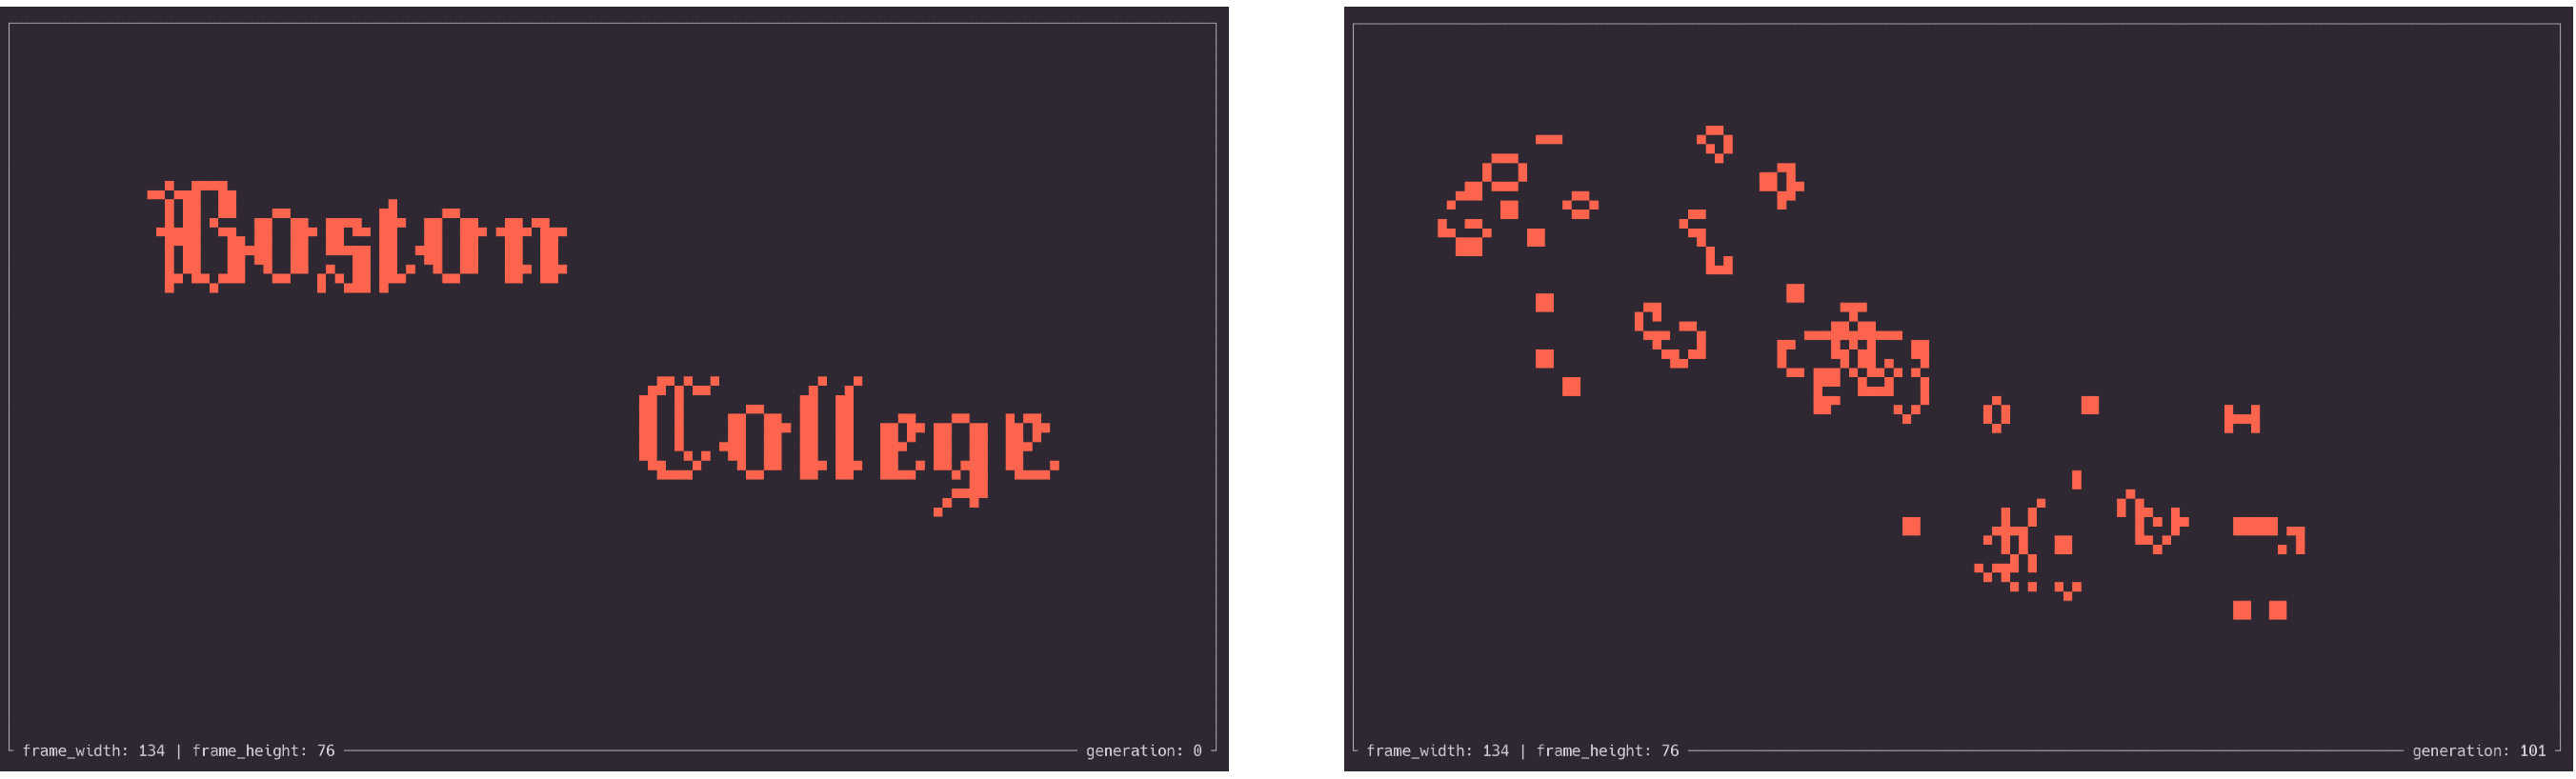
\includegraphics[width=16.5cm]{bc_figure.png}
    \caption{Game of Life Example on Starting Configuration ``Boston College" (Generation 0 to 101)}
\end{figure}


\subsection{The Game}
Similar to how Alan Turing proposed models of computational thinking prior to modern day computers, Conway's Game of Life started as a simple mathematical idea that was “played” on chalkboards and Go boards \cite{Izhikevich_Conway_Seth}. Here are the rules, and how to play: 

\

\textbf{Rules \& Properties: }
\begin{enumerate}
  \label{rules}
  \item \textbf{Domain: }\\ The automata in the game interact within an \textit{infinite} two-dimensional grid of cells. Every cell has eight neighbors \cite{Izhikevich_Conway_Seth}[see \ref{figure_one}]. \label{rule_one}

  \item \textbf{States: }\\ Each automata is represented independently by a single cell which can be either $\textit{alive}$ or $\textit{dead}$.

  \item \textbf{Initial Configuration: } \\ The beginning set of live or dead cells is determined or ``seeded" by the player prior to any evolution.

  \item \textbf{Evolution: } \\ The following rules are applied to all cells simultaneously in fixed time intervals called \textit{generations} \cite{Bontes2019}.

  \item \textbf{Birth: } \\ A new cell is born at generation $t + 1$ when its state is currently \textit{dead} and has exactly 3 lives neighbors (reproduction) \cite{Bontes2019}.

  \item \textbf{Death: } \\ Any currently living cell will die at generation $t + 1$ if it has less than 2 live neighbors (underpopulation) or more than 3 live neighbors (overpopulation) \cite{Bontes2019}.

  \item \textbf{Persistence: } \\ Any live cell will persist at $t + 1$ if it has 2 or 3 live neighbors at generation $t$ \cite{Izhikevich_Conway_Seth}.
\end{enumerate}

 \begin{figure}[ht]
          \centering
    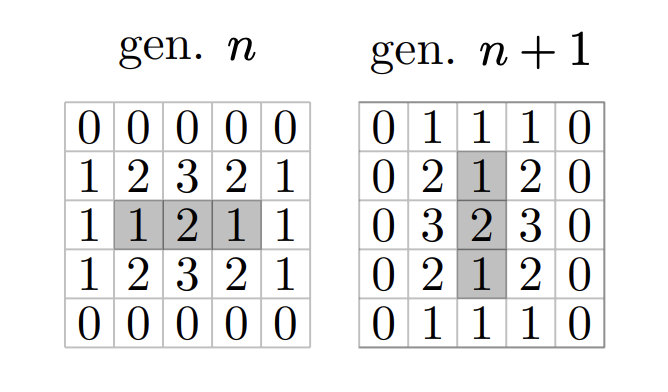
\includegraphics[width=8cm]{figures/figure_one.png}
    \caption{The evolution of a blinker from for 2 generations}
    \label{figure_one}
    \text{J. Bontes. “Searching for patterns in Conway’s Game of Life”}
    \cite{Bontes2019}
\end{figure}

It’s important to note that Conway’s Game of Life is not a game of how we traditionally think of games. There’s no objective, or winning or losing. They’re aren’t even any players – it is known to be a zero player game \cite{Beginning_Life_2006}. As technology advanced, Conway’s Game of Life proved to be well-suited for implementation on computers. Today, the game has been optimized to explore the many unresolved problems the game poses. 

\subsection{So... What's the Big Deal?}

At first glance, Conway’s Game of Life appears to be a simple simulation of cellular life based on just a few rules. However, beneath the surface, the Game hides complexity that has roused intense study since its public release way back in 1970. Decades have been spent examining the self-replicating machines, digital circuits, and unique patterns the Game presents. Another leading interest, of course, is the Game's overall mathematical complexity, which is the main inspiration of this paper. Additionally, many of GoL's difficulties also stem from the Game's Turing Completeness which we also will covered in this paper. 

\ 

\textbf{Proposal}: The purpose of this paper is to both synthesize concrete theoretical mathematics from Complexity Theory into a specific instance of Conway's game of life. More specifically, the paper will be divided into two parts. The first pertaining to the Pattern Reachability Question (\textbf{PREP}), and the second pertaining to Undecidability and Turing Completeness in the game.

\section {Pattern Reachability}
\label{patterns}
One particular challenge within The Game is the difficulty of predicting and discovering the many different patterns (or ``life-forms") that may evolve from one generation to the next. A\textit{ pattern} is defined as a constellation of both live and dead cells that evolve over time \cite{Bontes2019}.

\

Conway's Game of Life is capable of producing patterns that move back and forth, shifting between a finite set of states, patterns that traverse through the grid indefinitely, patterns that trail and leave behind other evolving patterns, and patterns that collide with each other to create other complicated patterns \cite{JG2022conway}.

\

Because of this, there are over a thousand different patterns and life-forms that have been proposed and studied within the Game (many of which are still be discovered today) \cite{Life_Wiki}. Of these many patterns, there are three underlying features that are used to categorize and study them. There are as follows: 

\begin{enumerate}
  \item \textbf{Still Life: } \\ A pattern that remains unchanged from one generation to the next \cite{JG2022conway}.

 \begin{figure}[ht]
          \centering
    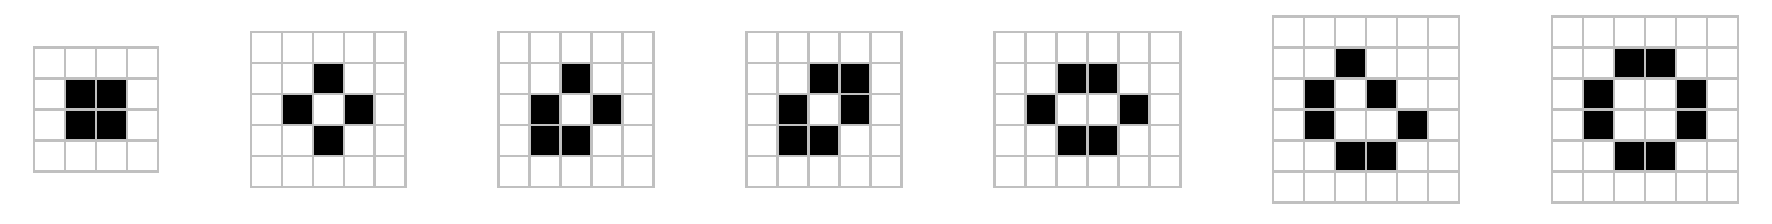
\includegraphics[width=10cm]{figures/figure_two.png}
    \label{stil_lifes}
    \caption{Examples of Still Lifes: From left to right: block, tub, boat, ship, beehive, loaf and pond}
    \text{Nathaniel Johnston and Dave Greene. Conway’s Game of Life: Mathematics and Construction.}
    \cite{JG2022conway}
\end{figure}


  \item \textbf{Oscillator: } \\ A pattern that cycles between finitely many different configurations. The configuration of the pattern within an individual generations is called a \textbf{phases}. The smallest number of generations needed to repeat the cycle is called the \textbf{period} \cite{JG2022conway}.



 \begin{figure}[ht]
          \centering
    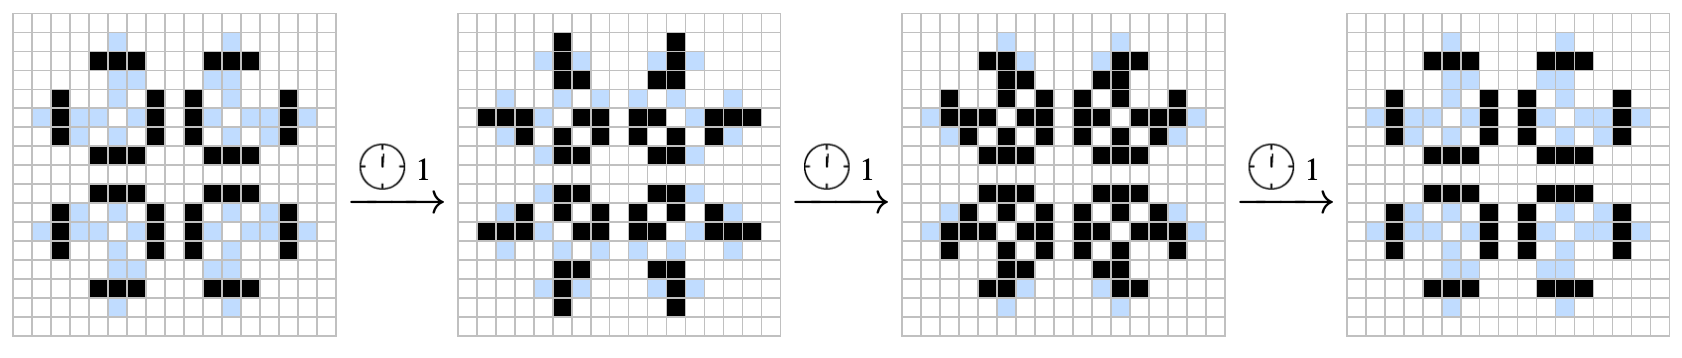
\includegraphics[width=14cm]{figures/figure_three.png}
    \caption{Period 3 Oscillator known as a Pulsar}
    \text{Nathaniel Johnston and Dave Greene. Conway’s Game of Life: Mathematics and Construction.}
    \cite{JG2022conway}
\end{figure}




\label{spaceship_def}
  \item \textbf{Spaceship: } \\ A pattern that returns to its initial phase after it completes its period, but ends in a different location from where it started. \cite{JG2022conway}
\end{enumerate}

 \begin{figure}[ht]
          \centering
    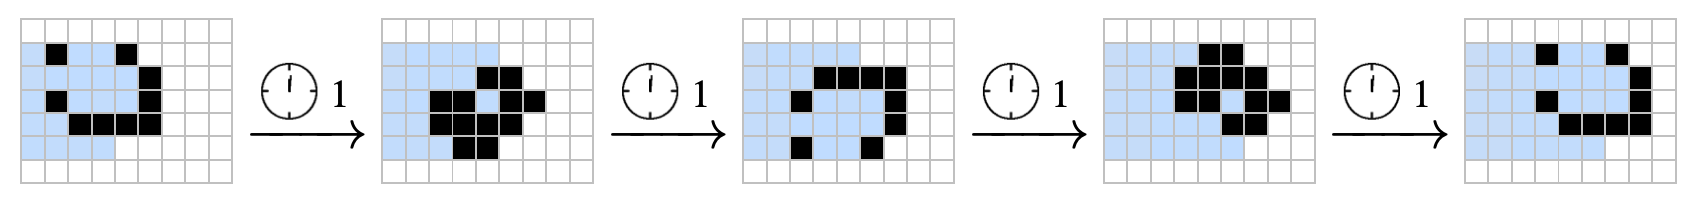
\includegraphics[width=15cm]{figures/figure_four.png}
    \caption{Period 4 Spaceship which moves orthogonally across the grid}
    \text{Nathaniel Johnston and Dave Greene. Conway’s Game of Life: Mathematics and Construction.}
    \cite{JG2022conway}
    \label{spaceship_figure}
\end{figure}


In defining the following life-forms, the next natural question to ask is: \textit{Given an initial starting configuration is it possible to decide if any Still Life, Oscillator, or Spaceship life-form patterns are reachable in t many generations?}

\

This question can be distilled down into a particular instance of the Pattern Reachability Problem (\textbf{PREP}) \cite{SUTNER199587}. The Pattern Reachability Problem asks: 

 \

 \textit{Question: } Given some instance of Conway's Game of Life, a cellular automata \textbf{GoL} [see \ref{gol}], a source configuration $X$ and a target configuration \textbf{$X_0$}, \textit{is there some configuration in the orbit of X that matches $X_0$, given $t$ generations pass?} \cite{SUTNER199587}.

\subsection{Definitions, Theorems, and other Important Terminology}
Before proving the proposition that 
\textit {PREP can be decided in nondeterministic polynomial time for two-dimensional finite automata in Conway's Game of Life} [see \ref{NP_proof}], lets first formulate the necessary definition, encodings, and terminology we'll need moving forward.

\subsection{Encoding cellular automata in Conway's Game of Life}
To begin, let's represent an instance of a cellular automata in Conway's Game of Life as a finite string over an alphabet. The following encoding is inspired by \textit{Sutner's} encoding scheme \cite{SUTNER199587}.
\begin{enumerate}
  \item[(a)] Let a CA in \textbf{GoL} be represented as a 4-tuple: \textbf{GoL = } $ \langle d, k, w, p \rangle$ \label{gol}
    \begin{enumerate}
      \item[-] $d$ denotes the dimensions of the \textbf{finite} grid that the automata evolve in. In representing Conway's game of life, our dimensions space will be set to $d = 2$
      \item[-] Every cell has a finite number of states, let's use a finite alphabet $\Sigma_k$, where $\Sigma_k = \{0,1\}$, $1$ indicating that a particular cell is \textit{living}, and $0$ indicating that that cell is \textit{dead}. Let $k$ represent this alphabet.
      \item[-] Positive integer $w$ represents the width of a automata's neighborhood in \textbf{GoL}, meaning \textit{the automata's direct neighbors that are involved in updating the cell}. Width is a result of the radius relation: $w = 2*r +1$. Within \textbf{GoL}, our neighborhood rules [rule: \ref{rule_one}], indicate $r = 1$, and $w = 3$.
      \item[-] Let $p : \Sigma^N \to \Sigma$ be the local function which expresses the formal rule mapping (or \textit{local rule}) of the automate in Conway's Game of Life. Our set of rules applies directly from the surrounding neighborsA $ N = [-r, r]^d \subseteq \mathbb{Z}^d $, and updates the cell in the center of the neighborhood.
      \item[-] A map $ X : C \to \Sigma $ takes the set $ C $ of all cells and maps to a state $ k \in \Sigma$. X is the \emph{configuration} of the cellular automaton.
    \end{enumerate}
      \item[(b)] The local map $p$ only updates a given automata based on it's direct neighbors. To extend this to the entire configuration $C$, let's define a global mapping $\rho$ which updates all cell simultaneously. This process will utilize our local mapping rule $p$, and  can be broken into two steps: 
        \begin{enumerate}
          \item[1).] For each cell $c \in C$ create it's local configuration $X_c$, which captures the neighbors around $c$.
          \item[2).] Apply the local rule $p$ to $X_c$ to get the new state at $c$.
        \end{enumerate}
        The global update rule $\rho : \Sigma^C \to \Sigma^C$ is  given by:
        \begin {equation}
        \rho(X)(c) = p(X_c)
        \end {equation}
      \item[(c)] In constructing a \textit{finite} instance of GoL, we must consider how cellular automata behavior on boundaries of the grid.
        \begin{enumerate}
          \item[-] To solve this problem, we will adopt \textit{fixed boundary conditions} \cite{SUTNER199587}. We'll assume that all cells that are not represented in our finite grid will have a fixed state set to $0$. In doing so we can redefine our local mapping $p$ slightly: 
          \item[-] Define $X_c(z)$ to be the state of a cell at postion $c + z$, whenever $c + z \in C$, define its state to be 0, if $c + z$ falls outside the grid.
        \end{enumerate}
      \item[(d)] Let's define the formal definition of a \textit{pattern}. \cite{SUTNER199587}
        \begin{enumerate}
           \item[-] A pattern is a partial configuration, defined as a map $X_0: C_0 \to \Sigma$, where $C_0 \subseteq C$.
    \item[-] We say that a configuration $X$ matches pattern $X_0$ if $X(c) = X_0(c)$ for all $c \in C_0$.
        \end{enumerate}

\item[(e)] The \textit{orbit} of a configuration $X$ is another important definition in regard to our Pattern Reachability Question. The \textit{orbit} is the full set of all intermediary states the system ever passes through starting from $X$. Formally, the orbit is defined as

\begin{equation}
  \text{Orbit of } X = \{ X, \rho(X), \rho^2(X), \rho^3(X), \dots \}
\end{equation}

Another, more useful way we'll be using \textit{orbit} will in regard to some $t$ that is: 

\begin{equation}
\text{Orbit}(X) = \{ \rho^t(X) \mid t \geq 0 \}
\end{equation}

where \( \rho \) is the global update rule and \( t \) ranges over the non-negative integers.
\end{enumerate}
\section{Pattern Reachability}
Now that we have built out the formal definition of \textbf{GoL} automata, we can treat the Pattern Reachability question as a decision problem that uses our \textbf{GoL} definitions. To prove that \textbf{PREP} $\in$ \textbf{NP}, let's begin by expressing \textbf{PREP} more formally as a decision problem: \textit{Does there exist a time $t \geq 0$ such that the configuration $\rho^t(X)$ contains a given pattern $X_0$?}

\subsection{PREP is in NP:}

\label{NP_proof}
\textit{Let's prove by constructing a certificate based definition}\\
\\
\textbf{Problem Input:}
\begin{itemize}
  \item An instance of \textbf{GoL} automata: $ \langle d = 2, \Sigma_k = \{0,1\}, w = 3, p = \text{(local rule)} \rangle$
    \item Finite grid configuration $ C$, where $ |C| $ is the total number cells $n$.
  \item Initial configuration $ X: C \to \Sigma_k = \{0,1\}$ 
    \item Target pattern $ X_0: C_0 \to \Sigma_k $ where \( C_0 \subseteq C \)
\end{itemize}

\subsubsection{NP Certificate Based Proof:\cite{SUTNER199587}}
We say a  Language \textbf{L} $\in$ \textbf{NP} if there exists a polynomial-time TM that can verify \textbf{PREP}'s certificate efficiently. Let's begin by constructing the certificate (nondeterministicically guessing the solution to \textbf{PREP}).

\begin{enumerate}
    \item \textbf{Certificate:} A tuple $Z = \langle t, X_0 \rangle$
      Where: 
      \begin{enumerate}
          \item[(a)] $t$ is a non-negative integer that represents the number of configuration states 
          \item[(b)]) $X_0$ represents the target pattern configuration $\rho^t(X)$ should produce after $t$ configuration states.
      \end{enumerate}
    \item \textbf{Verification process} Given tuple $Z$:
    \begin{enumerate}
        \item Begin by simulating GoL for $t$ steps. Start with configuration $X$, compute $\rho^t(X)$ (the \textit{orbit} of $X$).
        \begin{itemize}
            \item Apply our Local update rule: For each cell $c \in C$, compute its next state based on surrounding neighborhood. Each cell is able to apply the local rule in constant time: $O(1)$
            \item To update all $n$ cells in configuration, this takes $n*O(1)$ or $O(n)$ time. This our ``per-step" time.
            \item Total compute time for $t$ steps is: $O(t * n) = O(n * t)$
        \end{itemize}
        \item Now we must Check to see if resulting configuration matches, that is, we must verify $\rho^t(X)$  matches $X_0$ on $C_0$:
        \begin{itemize}
            \item For each cell $c \in C_0$ check if $\rho^t(X)(c) = X_0(c)$.
            \item This checking must be done for $ |C_0| \leq n $ cells, which takes time: $ O(n) $.
        \end{itemize}
    \end{enumerate}

    \item \textbf{Total verification time: }
      \begin{equation}
        O(t*(n)*n)+O(n)= O(t *n^2) \in \textbf{P} 
    \end{equation}
    \textit{For any} $t$ \textit{in polynomial time}.
  \item[]\textbf{Analysis:}
    The orbit of the initial configuration $X$ under repeated application of our global update rule $\rho$ describes all possible future sub-states the configuration. Our certificate claims that at some guessed $t$ value the configuration $\rho^t(X)$ will represent the desired pattern $X_0$. More specifically, since we can compute the orbit in $t$ steps and check if the resulting configuration matches $X_0$ in polynomial time, \textbf{PREP} $\in$ \textbf{NP}.
\end{enumerate}

\subsection{Still Life, Oscillator, and Spaceship Pattern Reachability}

\textbf{Let's now apply the proof above to particular instances of common patterns in GoL}
In any each case we start be expressing the target pattern as a partial configuration
\begin{equation}
  X_0 \colon C_0 \to \{0,1\},
\end{equation}
Our decision question remains the same: $\exists\,t\ge0:\ \rho^t(X)$ produces a configuration which is equal to $X_0$?.

\
\

\textbf{Still Life analysis:}
Our proof [\ref{NP_proof}] applies most directly for the still life patterns. That is, we can define our target pattern as one of the particular Still life forms [see figure \ref{stil_lifes}], then check for some nondeterministicically guessed $t$: 
\begin{equation}
  \rho^t(X)(c) = X_0(c)\quad\forall\,c\in C_0.
\end{equation}

\paragraph{Oscillator analysis:} 
What about for patterns that change from state $t$ to state $t+1$? In other words, how can we apply our NP proof for oscillating patterns that cycle every period $p$. In this case, we can begin the proof much of the same way, but check to see if each pattern that cycles in period $p$ is satisfiable. The decision problem then becomes the Conjunctive Normal Form of all all patterns that make up the oscillating period. We can express this as:


\begin{equation}
\textbf{PREP}(\langle t, X_{0,p=0} \rangle) \land \textbf{PREP}(\langle t+1, X_{0,p=1} \rangle) \land \cdots \land \textbf{PREP}(\langle t+n, X_{0,p=p_n} \rangle)
\end{equation}

Where $p_n$ represents each of the $n$ phases that make up the oscillator. An oscillating pattern is reachable if and only if all phases are reachable at configuration $t$, and for the next $n$ phases.

\
\

\textbf{Spaceship analysis:}
As per our definition of Spaceships [see \ref{spaceship_def}], Spaceships are much like oscillators, but after each generation in their period $p$, the whole pattern translates to a new position (from generation $t$ to $t+1$). We can model this translation with a shifting coordinate rule $v = (x,y)$, where $x$ represents the shifting amount on the x-axis, and $y$ on the y-axis, so long as $x,y \leq$ max grid dimensions. Let's model the following using our Period 4 Spaceship example from Figure 5 [see \ref{spaceship_figure}].This particular Spaceship always moves in the positive x direction, and alternates between moving in the positive and negative y direction. We can model this Pattern by using the translation rule $v = (1,\pm1)$. Let's now express the full CNF:


\begin{equation}
  \textbf{PREP}(\langle t, X_{0,p=0,v=(1,-1)} \rangle) \land \textbf{PREP}(\langle t+1, X_{0,p=1,v=(1,1)} \rangle) \land \cdots \land \textbf{PREP}(\langle t+n, X_{0,p=n,v=(1,\pm1)} \rangle)
\end{equation}

Just as before, a Spaceship pattern in reachable iff all phases are reachable at configuration $t$, and for the next $n$ phases (while also accounting for shift rule $v$).

\section{What can be computed/decided in Conway’s Game of Life?}

% TODO: add personality..improve flow w.r.t. now made sections
% no need to rehash turing complete
The quest to understand the limits of computation has been a central theme in computer science since its inception. Alan Turing's groundbreaking work introduced the concept of a theoretical machine, now known as the Turing machine (TM), capable of simulating any algorithm. As we talked about in class, systems that possess this capability are deemed \textit{Turing complete}, signifying they have the maximum theoretical computational power. Discovering that a system, especially one with seemingly simple rules like Conway's Game of Life, is Turing complete reveals a profound depth and complexity. It implies that the system can, in principle, compute anything that any other computer can. This section delves into the remarkable computational capabilities embedded within the evolving patterns of Conway's Game of Life, exploring how complex computational structures, including Turing machines themselves, can emerge from its basic local interactions.

In short, we'll provide an overview of how it's even possible to construct a Universal Turing machine (UTM) in Life, and why that validates it as a Turing complete model of computation.

\subsection{Gliders}

A \textit{glider} is a specific pattern in Conway's Game of Life that exhibits translational movement across the grid while undergoing periodic transformations in its structure. Formally, we define a glider as follows:

\begin{definition}[Glider]
A glider is a configuration $G$ of live cells in Conway's Game of Life such that:
\begin{enumerate}
    \item After exactly $p$ generations (where $p = 4$), the pattern transforms into a translated version of itself: $G_{t+p} = T(G_t)$, where $T$ represents a translation operation.
    \item The translation $T$ corresponds to a diagonal movement by one cell diagonally (specifically, $\pm 1$ cell horizontally and $\pm 1$ cell vertically).
    \item The pattern consists of exactly 5 live cells in each of its phase configurations.
    \item The pattern cycles through exactly 4 distinct configurations before returning to a translated version of its initial state.
\end{enumerate}
\end{definition}

As illustrated in Figure \ref{fig:glider-generations}, the glider completes a full cycle every 4 generations, moving one cell diagonally in the process. The minimal glider discovered by Conway consists of 5 live cells arranged in an asymmetric pattern that evolves through 4 distinct phases before returning to its original configuration, albeit in a new position.

\begin{figure}[H]
  \centering
  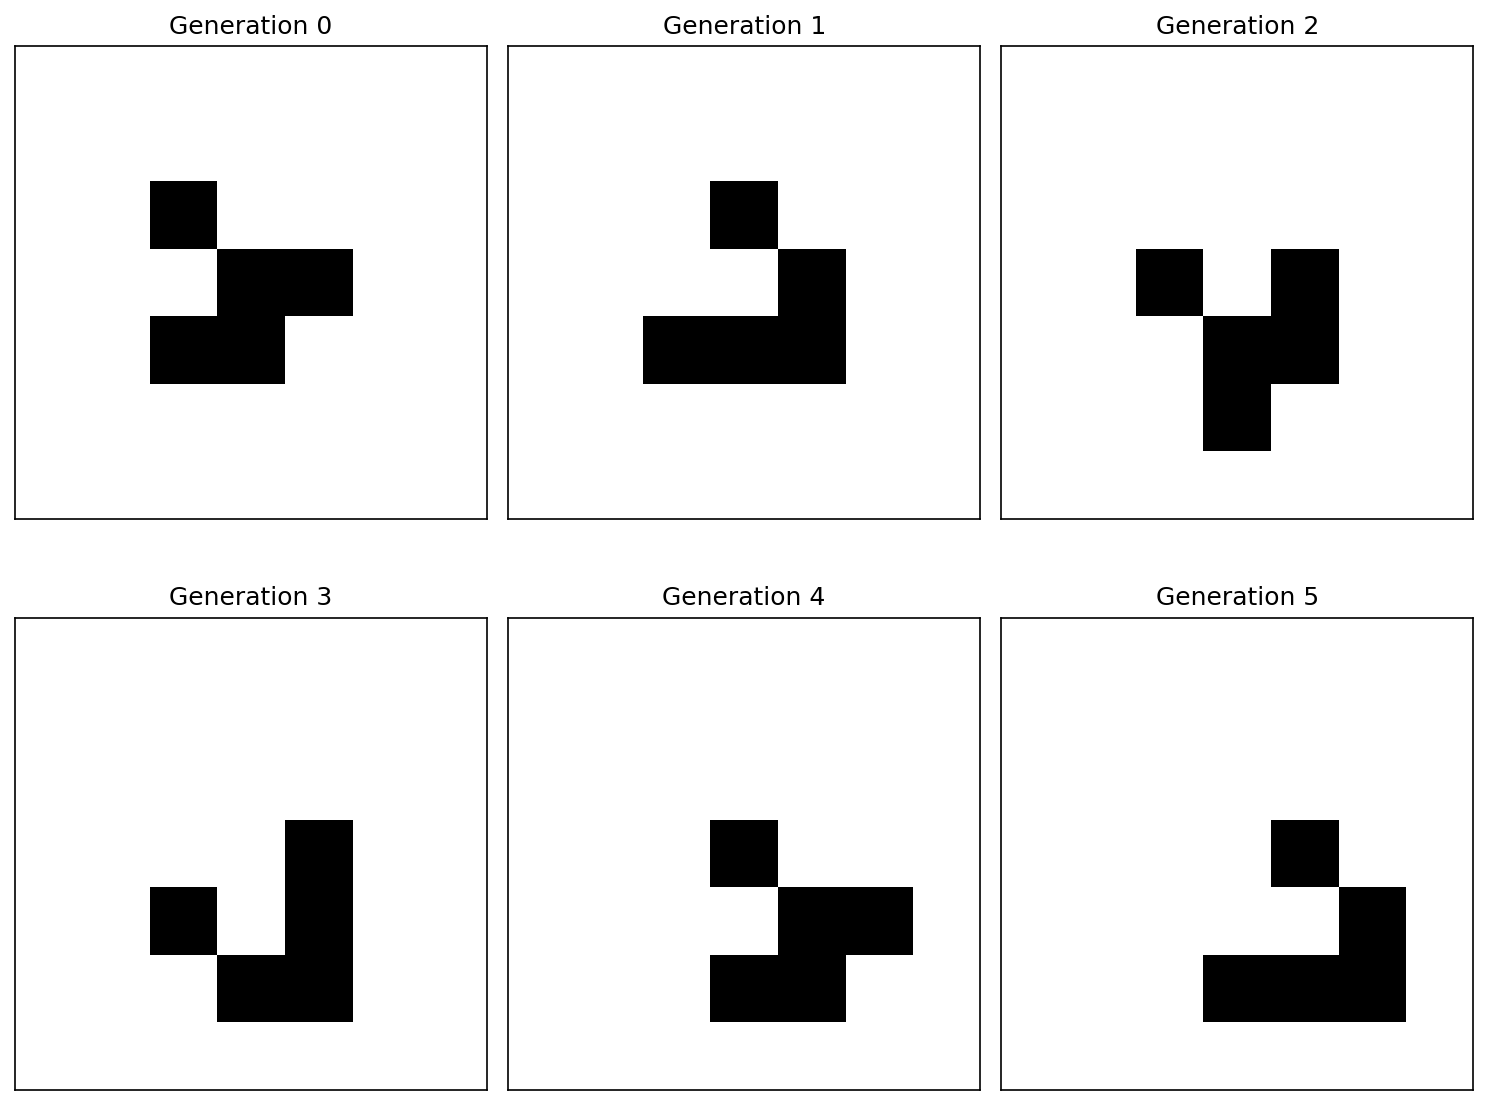
\includegraphics[width=0.8\textwidth]{figures/glider_generations_0_to_5.png}
  \caption{Evolution of a glider pattern through generations 0 to 5, demonstrating the characteristic diagonal movement and shape cycle.}
  \label{fig:glider-generations}
\end{figure}

Gliders are particularly significant in Conway's Game of Life because they serve as the fundamental mechanism for information transfer, as we'll see in the next few sections. Since they can travel arbitrarily far across the infinite grid, they effectively function as signals or "data packets" in computational constructions. In order to talk about operations on such "data" later on, we'll also need to define the following:

\begin{definition}[Glider Collision]
Let $G_1$ and $G_2$ be glider patterns with positions $P_1(t)$ and $P_2(t)$ at time $t$, where $P_i(t)$ denotes the set of coordinates of live cells comprising glider $G_i$. A glider collision occurs at time $t_c$ if there exists a time $t_c$ such that:
\begin{enumerate}
  \item For all $t < t_c$, the evolution of $G_1$ and $G_2$ proceeds independently, i.e., the state of each cell at time $t$ depends only on its own glider pattern's evolution.
  \item At time $t_c$, there exists a neighborhood $N$ such that both gliders influence the evolution of cells in $N$, formally: $\exists N \subseteq \mathbb{Z}^2$ such that $d(P_1(t_c), N) \leq 1$ and $d(P_2(t_c), N) \leq 1$, where $d$ denotes minimum Manhattan distance.
\end{enumerate}

The outcome of a collision at time $t_c+k$ (for some finite $k > 0$) can be classified as one of:
\begin{enumerate}
  \item \textit{Annihilation}: The resulting pattern $R(t_c+k)$ contains no persistent structures, i.e., $\exists t' > t_c+k$ such that $\forall t > t'$, $R(t) = \emptyset$.
  \item \textit{Reflection}: The resulting pattern contains exactly two gliders $G'_1$ and $G'_2$ with velocity vectors $v'_1$ and $v'_2$ such that $v'_i \neq v_i$ for at least one $i \in \{1,2\}$.
  \item \textit{Transformation}: The resulting pattern contains at least one glider with a velocity vector different from both $v_1$ and $v_2$, or the number of resulting gliders differs from the initial number.
  \item \textit{Creation}: The resulting pattern contains both one or more gliders and at least one persistent non-glider structure (still life or oscillator).
\end{enumerate}
\end{definition}

% figure
% make an animation for each?

Glider collisions, depending on their precise timing and geometry, can be engineered to perform logical operations, redirect glider streams, or even annihilate them. This controlled interaction forms the basis for constructing logic gates and memory elements, essential components for the computation we'll be discussing. Consequently, the final bit of glider-oriented prep/background we'll do here is defining a generator of gliders itself, known as a \textit{glider gun}.

\begin{definition}[Glider Gun]
A pattern $G \subseteq \mathbb{Z}^2$ is a glider gun with period $p \in \mathbb{Z}^+$ if there exists a finite core region $C \subseteq \mathbb{Z}^2$ and a sequence of configurations $(G_t)_{t=0}^{\infty}$ representing the evolution of $G$ under Conway's Game of Life rules such that:
\begin{enumerate}
  \item There exists a non-empty finite set $C \subseteq G$ such that $\forall t \geq 0$, $G_t \cap C = G_{t+p} \cap C$
  
  \item There exists a sequence of times $(t_n)_{n=1}^{\infty}$ with $t_n = np + d$ for some fixed offset $d \in \{0, 1, \ldots, p-1\}$ and a glider pattern $H$ such that:
    \begin{itemize}
      \item For each $n \geq 1$, there exists a translation vector $\vec{v}_n = n \cdot \vec{v}$ for some fixed $\vec{v} \in \mathbb{Z}^2 \setminus \{(0,0)\}$ such that $H + \vec{v}_n \subseteq G_{t_n}$
      \item For any distinct $n, m \geq 1$, the patterns $H + \vec{v}_n$ and $H + \vec{v}_m$ are disjoint
    \end{itemize}
    
  \item There exists $T \in \mathbb{Z}^+$ such that for all $n \geq 1$ and all $t \geq t_n + T$, the evolution of $H + \vec{v}_n$ proceeds independently of both the core region $C$ and all other emitted gliders
  
  \item The distance between the core region $C$ and the $n$-th emitted glider $H + \vec{v}_n$ increases without bound as $n \to \infty$
\end{enumerate}
\end{definition}

\begin{figure}[H]
  \centering
  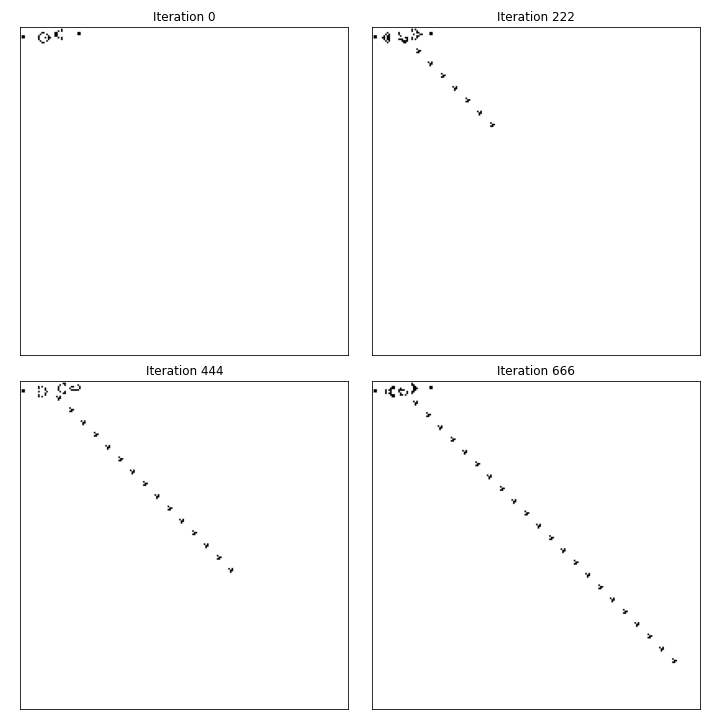
\includegraphics[width=0.8\textwidth]{figures/gosper_gun_iterations.png}
  \caption{The Gosper Glider Gun, discovered in 1970 by Bill Gosper, continually fires gliders in one of 4 diagonal directions. The above shows a Gosper Glider Gun firing southeast for 666 generations.}
  \label{fig:gosper-gun}
\end{figure}


\subsubsection{Essential Circuit Components: Eaters, Reflectors, and Other Functional Patterns}
In constructing computational circuits within Conway's Game of Life, several specialized patterns beyond basic gliders and logic gates are essential. These functional patterns serve as the "supporting infrastructure" for complex computational architectures, managing glider traffic, terminating signals, and redirecting information flows.
We won't be so rigorous as to worry about individual implementations of these components in our constructions, but note that they act as the links between our gates.\footnote{look at the page count...}While the detailed implementation of these components is fascinating from an engineering perspective, focusing on them would distract from our primary goal of demonstrating the theoretical computational power of Life. Readers interested in specific implementations may refer to Paul Rendell's comprehensive work on Life components or Adam Goucher's "Game of Life Glider Construction Kit."

\begin{definition}[Eater]
An \textit{eater} is a stable pattern that can absorb (or "eat") specific incoming patterns, typically gliders, without being permanently altered. Formally, an eater $E$ is a pattern with the following properties:
\begin{enumerate}
  \item $E$ is a stable pattern (still life) that persists indefinitely when isolated.
  \item When a pattern $P$ (typically a glider) collides with $E$ at specific positions and orientations, $P$ is completely eliminated.
  \item After the collision and a finite number of generations, $E$ returns to its original configuration.
\end{enumerate}
\end{definition}

The most common eater, known as "eater 1," is a 7-cell still life that can absorb gliders arriving from specific directions. Eaters serve as "signal terminators" in computational circuits, cleanly removing gliders that have completed their function without generating debris that might interfere with other components.

\begin{figure}[H]
  \centering
  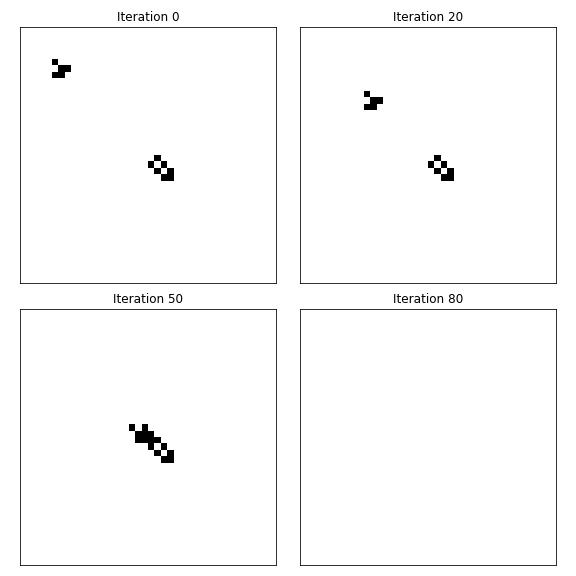
\includegraphics[width=0.6\textwidth]{figures/eater_interaction_iterations.png} % Placeholder for image
  \caption{An eater absorbing an incoming glider.}
  \label{fig:eater}
\end{figure}

\begin{definition}[Reflector]
A \textit{reflector} is a pattern that changes the trajectory of a glider (or other traveling pattern) without being permanently altered. A reflector $R$ satisfies:
\begin{enumerate}
  \item When a glider $G$ with velocity vector $\vec{v}$ collides with $R$ at specific positions and orientations, a glider $G'$ emerges with a different velocity vector $\vec{v}'$ (typically perpendicular to $\vec{v}$).
  \item After the collision and a finite number of generations, $R$ returns to its original configuration.
\end{enumerate}
\end{definition}

Common reflectors include the "glider reflector" (which performs 90° turns) and the "buckaroo" (which can redirect gliders 180°). Reflectors are crucial for routing glider signals through complex circuit layouts, allowing single-direction gliders to navigate two-dimensional paths.

\begin{figure}[H]
  \centering
  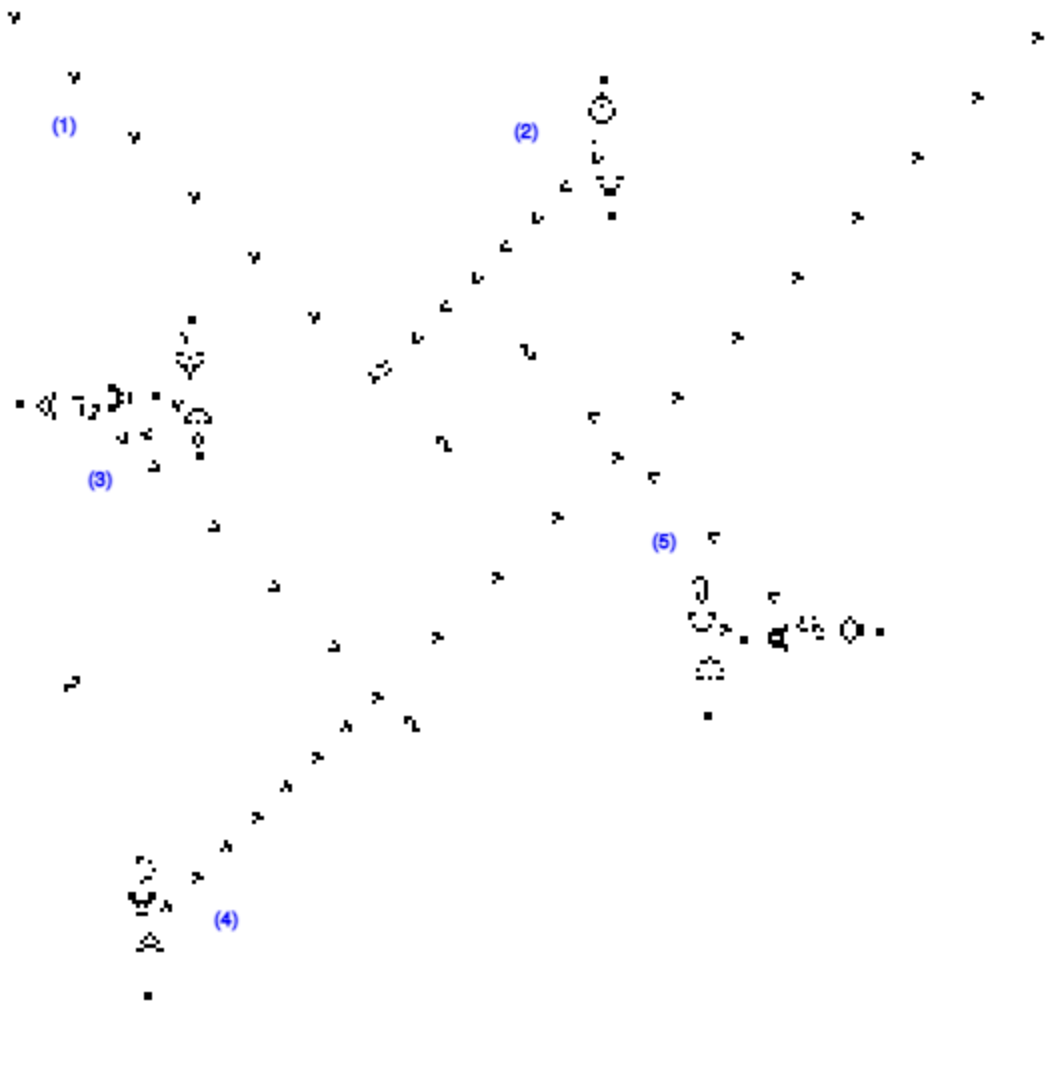
\includegraphics[width=0.6\textwidth]{figures/rotator.png} % Placeholder for image
  \caption{An southeast input stream of gliders (1), being rotated 90º ccw and outputted as a northeast output stream (4) \cite{Carlini_2020}}
  \label{fig:rotator}
\end{figure}

\begin{definition}[Signal Conditioner]
A \textit{signal conditioner} is a pattern arrangement that modifies glider streams in useful ways, including:
\begin{enumerate}
  \item \textbf{Duplicators:} Patterns that split a single input glider into multiple output gliders traveling in different directions.
  \item \textbf{Filters:} Configurations that selectively allow gliders through based on timing or spacing, removing gliders from a stream at specific intervals.
  \item \textbf{Delay Lines:} Arrangements that introduce precise timing delays to synchronize different glider streams. These typically consist of longer paths with additional reflectors.
\end{enumerate}
\end{definition}

\begin{definition}[Circuit Stabilization Patterns]
\textit{Circuit stabilization patterns} are auxiliary structures placed within computational circuits to:
\begin{enumerate}
  \item Absorb potentially damaging debris from nearby interactions.
  \item Prevent unwanted pattern growth from extending into critical areas.
  \item Maintain clean boundaries between functional components.
  \item Provide structural stability to nearby oscillators or other dynamic elements.
\end{enumerate}

These include strategically placed blocks, beehives, loaves, and other still lifes that serve as "insulators" or "guardrails" for active components.
\end{definition}

The integration of these specialized functional patterns enables the construction of reliable, complex computational circuits within Conway's Game of Life. Eaters terminate unwanted signals, reflectors direct information flow, and signal conditioners manage the timing and routing of glider streams. Together with the logic gates discussed previously, these components form the complete "toolbox" necessary for engineering universal computational systems. In practice, large-scale constructions (like those we'll talk about later) employ thousands of these patterns arranged with precise spatial and temporal relationships, forming a computational architecture that transcends the simple local rules of the cellular automaton.



\subsection{A Turing Machine in Life}

% Outline for Section: A Turing Machine in Life

% This section aims to bridge the gap between the basic elements like gliders 
% and the complex assertion that Life is Turing complete by outlining the 
% construction of a Turing machine within the game.
In showing that Life is Turing Complete, a nice first step will be to show that a TM can be constructed in Life. Let's do that..

\subsubsection{Logic Gates from Glider Collisions}

Having established the existence of gliders as mobile information carriers and glider guns as sources for these carriers, we now explore how interactions between gliders can be engineered to perform fundamental logical operations. The core idea is to represent binary information using the presence or absence of gliders within precisely timed streams.

\begin{definition}[Glider Stream Representation of Binary Signals]
Let $P$ be a fixed spatial path (typically a straight line or a sequence of connected line segments) and $v$ be the velocity vector of a standard glider along this path. A \textit{glider stream} along $P$ is a sequence of potential glider positions $(p_i)_{i=0}^{\infty}$ such that $p_{i+1} = p_i + v \cdot \Delta t$ for a fixed time interval $\Delta t$. A binary sequence $(b_i)_{i=0}^{\infty}$, where $b_i \in \{0, 1\}$, is represented by this glider stream as follows:
\begin{itemize}
  \item If $b_i = 1$, a glider exists at position $p_i$ at time $t_i = i \cdot \Delta t + t_0$ (for some initial time $t_0$).
  \item If $b_i = 0$, no glider exists at position $p_i$ at time $t_i$.
\end{itemize}
We refer to the presence of a glider at the expected time and position as a logical '1' signal, and its absence as a logical '0' signal.
\end{definition}

With this representation, we can construct logic gates by arranging collisions between glider streams such that the output stream (presence or absence of a glider at a specific time and location) corresponds to the desired logical function of the input streams.

\begin{definition}[Glider-Based Logic Gate]
A glider-based logic gate for a Boolean function $f: \{0, 1\}^n \to \{0, 1\}$ is a configuration $C$ in Conway's Game of Life involving $n$ input glider streams $S_{in,1}, \dots, S_{in,n}$ and one output glider stream $S_{out}$ such that:
\begin{enumerate}
  \item The streams are spatially and temporally arranged such that gliders (if present according to the input binary values $b_1, \dots, b_n$) collide within a specific interaction region derived from $C$.
  \item The state of the output stream $S_{out}$ at a designated time $t_{out}$ (representing the presence or absence of a glider) corresponds precisely to the value $f(b_1, \dots, b_n)$.
  \item The interaction mechanism must function correctly for all $2^n$ possible input combinations.
  \item The gate should ideally be resettable or operate continuously without interference between consecutive operations (though this often requires careful timing and spacing).
\end{enumerate}
\end{definition}

We now outline the conceptual construction of basic gates:

\paragraph{NOT Gate:} A NOT gate requires one input stream and one output stream. A common construction involves the input glider stream colliding with a specific stable or oscillating pattern (sometimes generated by an auxiliary glider gun).
\begin{itemize}
  \item \textbf{Input '1' (Glider Stream Present):} The input glider collides with the pattern in such a way that both are annihilated, or the glider is deflected away from the output path. Result: No glider emerges on the output path (Output '0').
  \item \textbf{Input '0' (Glider Absent):} No collision occurs. A separate, synchronized glider (often called a 'clock' or 'enable' glider), which would normally be destroyed by the input '1' glider, is allowed to pass through to the output path. Result: A glider emerges on the output path (Output '1').
\end{itemize}

\begin{figure}[H]
  \centering
  \begin{minipage}{0.45\textwidth}
    \centering
    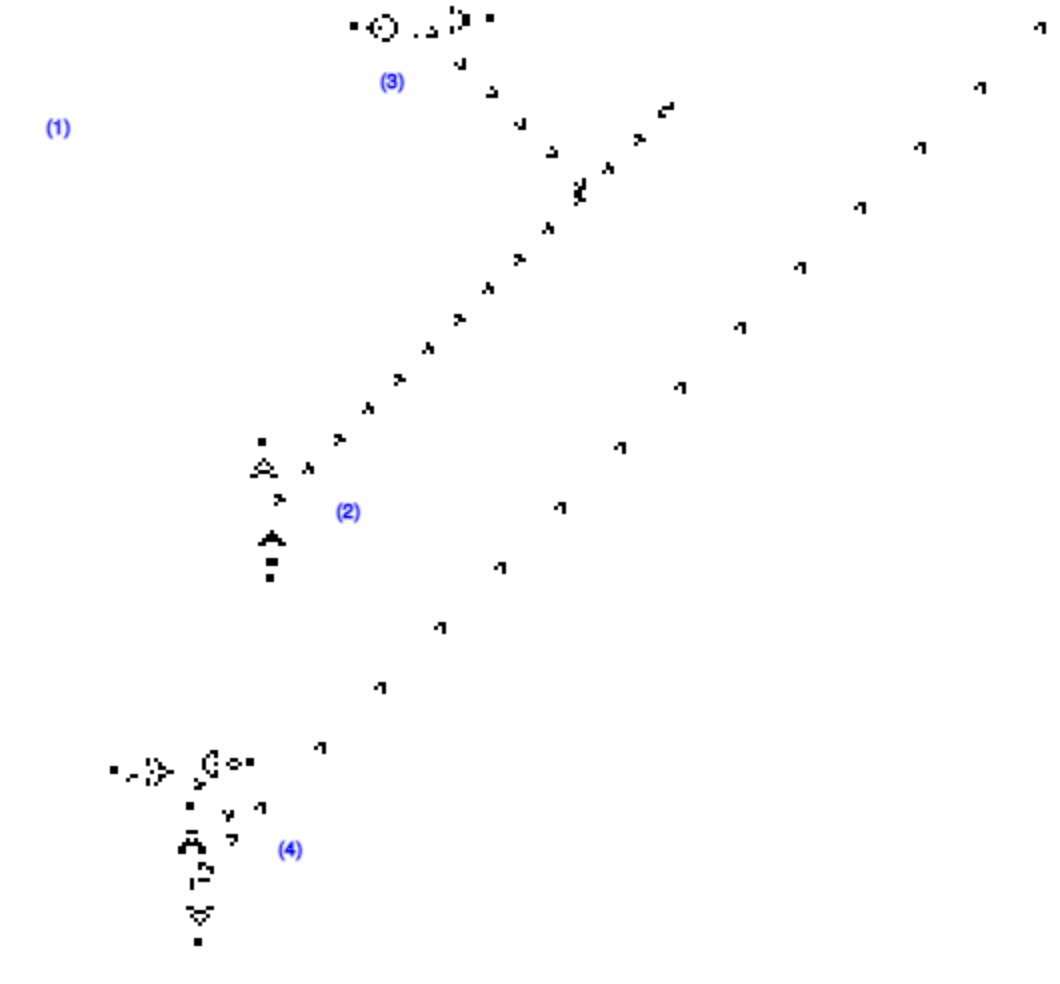
\includegraphics[width=\linewidth]{figures/notGo.png}
  \end{minipage}\hfill
  \begin{minipage}{0.45\textwidth}
    \centering
    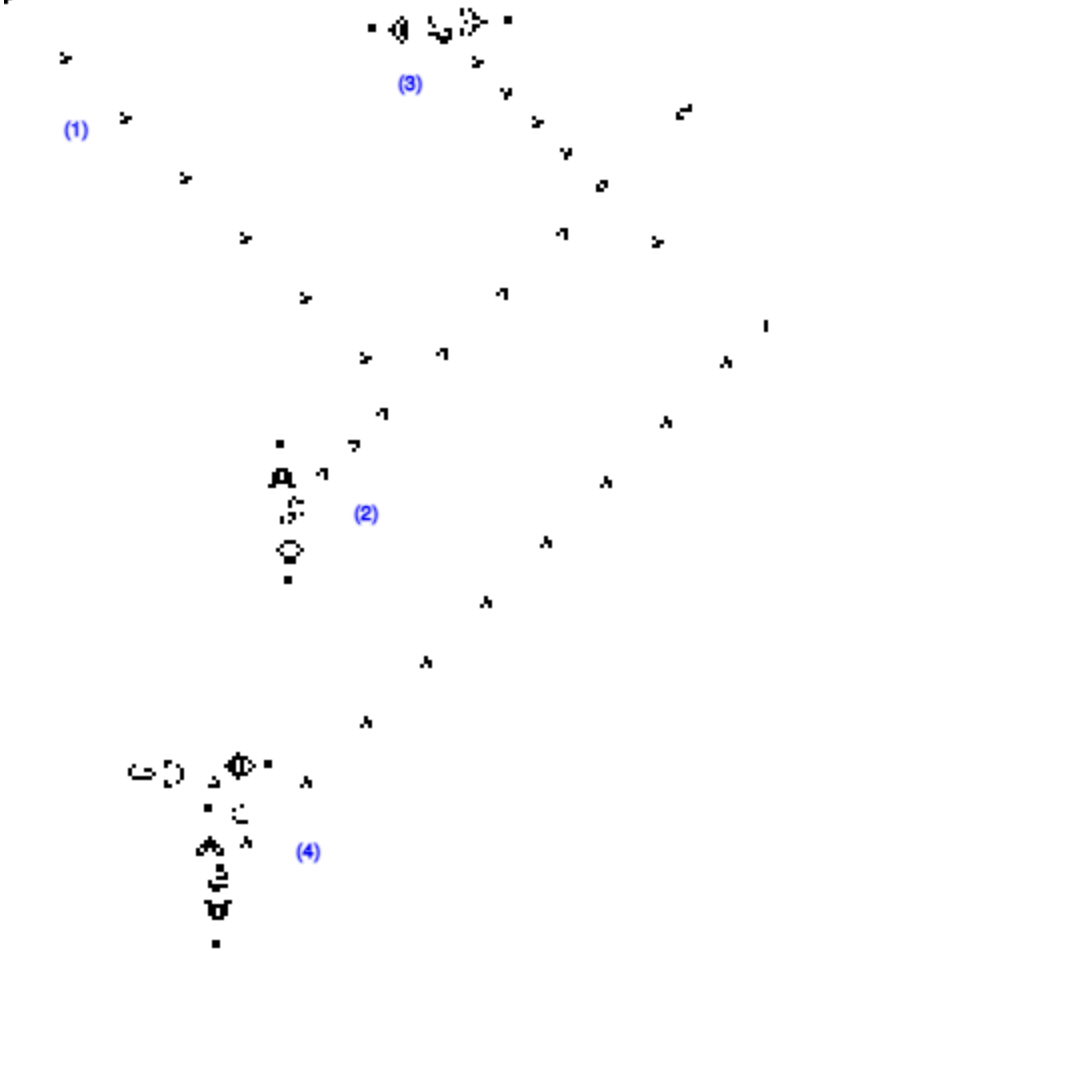
\includegraphics[width=\linewidth]{figures/notNoGo.png}
  \end{minipage}
  \caption{Left: Input stream (1) is inactive, making output stream (4) active. Right: Input stream (1) is active, making output stream (4) active. \cite{Carlini_2020}}
  \label{fig:not-gate-collision} % Changed label slightly to avoid conflict if fig:not-gate is used elsewhere
\end{figure}
This requires precise synchronization between the input stream and the auxiliary pattern or glider.

\paragraph{AND Gate:} An AND gate requires two input streams ($S_{in,1}, S_{in,2}$) and one output stream ($S_{out}$). The collision geometry is designed such that:
\begin{itemize}
  \item \textbf{Input ('1', '1'):} Gliders from both $S_{in,1}$ and $S_{in,2}$ arrive simultaneously (or with precise timing offset) at the interaction region. Their collision is engineered (potentially involving intermediate reactions or helper patterns) to produce exactly one glider directed onto the $S_{out}$ path. Result: Output '1'.
  \item \textbf{Input ('1', '0') or ('0', '1'):} Only one glider arrives. The collision geometry ensures that a single incoming glider is either destroyed, deflected away from $S_{out}$, or passes through harmlessly along a path different from $S_{out}$. Result: Output '0'.
  \item \textbf{Input ('0', '0'):} No gliders arrive. No reaction occurs. Result: Output '0'.
\end{itemize}
Achieving the specific ('1', '1') $\to$ '1' outcome while ensuring all other cases yield '0' requires intricate collision engineering. Many known constructions rely on sequences of specific glider collisions.

\begin{figure}[H]
  \centering
  % Case 00 -> 0
  \begin{minipage}{0.45\textwidth}
    \centering
    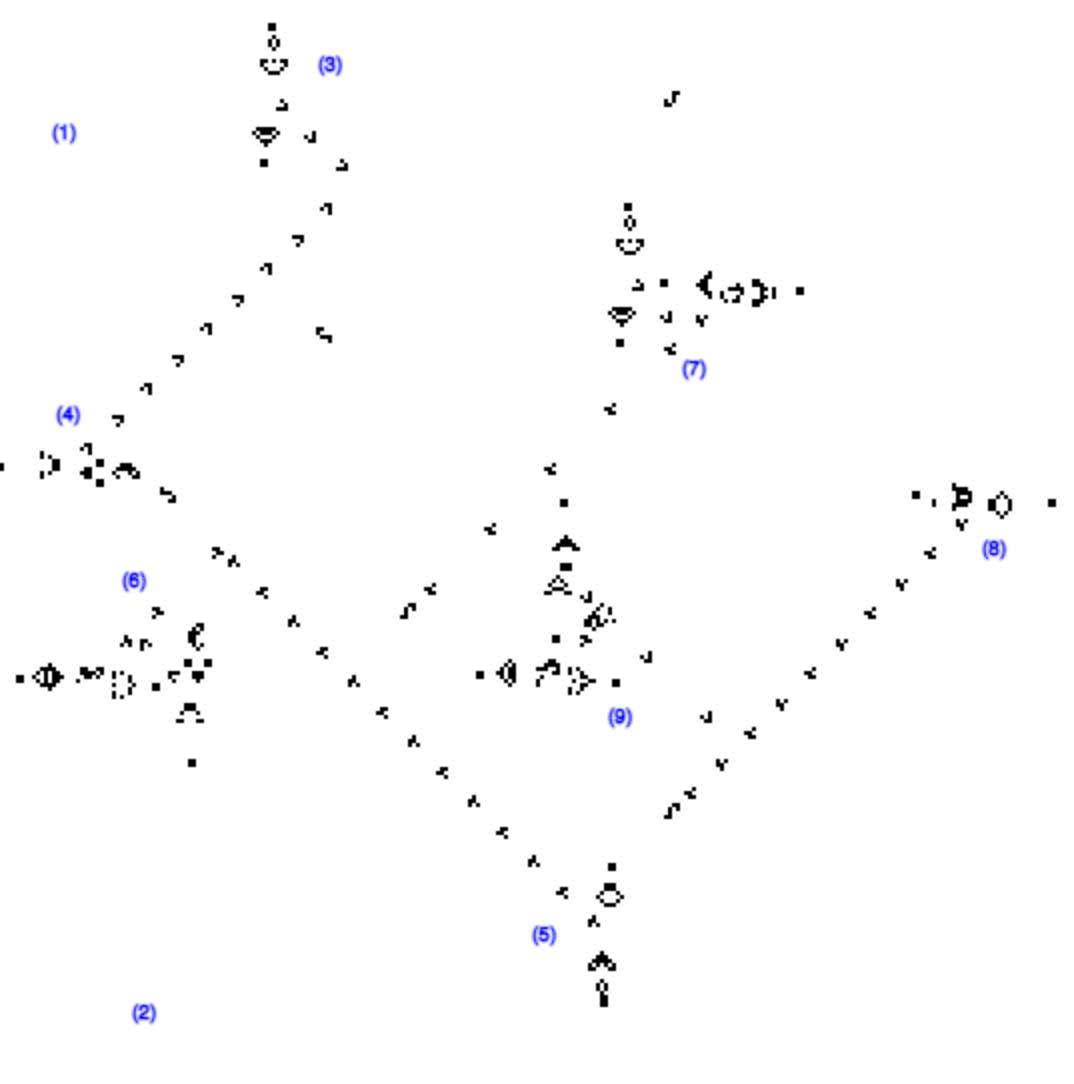
\includegraphics[width=\linewidth]{figures/andNoGo12.png} % Placeholder - Replace with actual image if available
  \end{minipage}\hfill
  % Case 01 -> 0
  \begin{minipage}{0.45\textwidth}
    \centering
    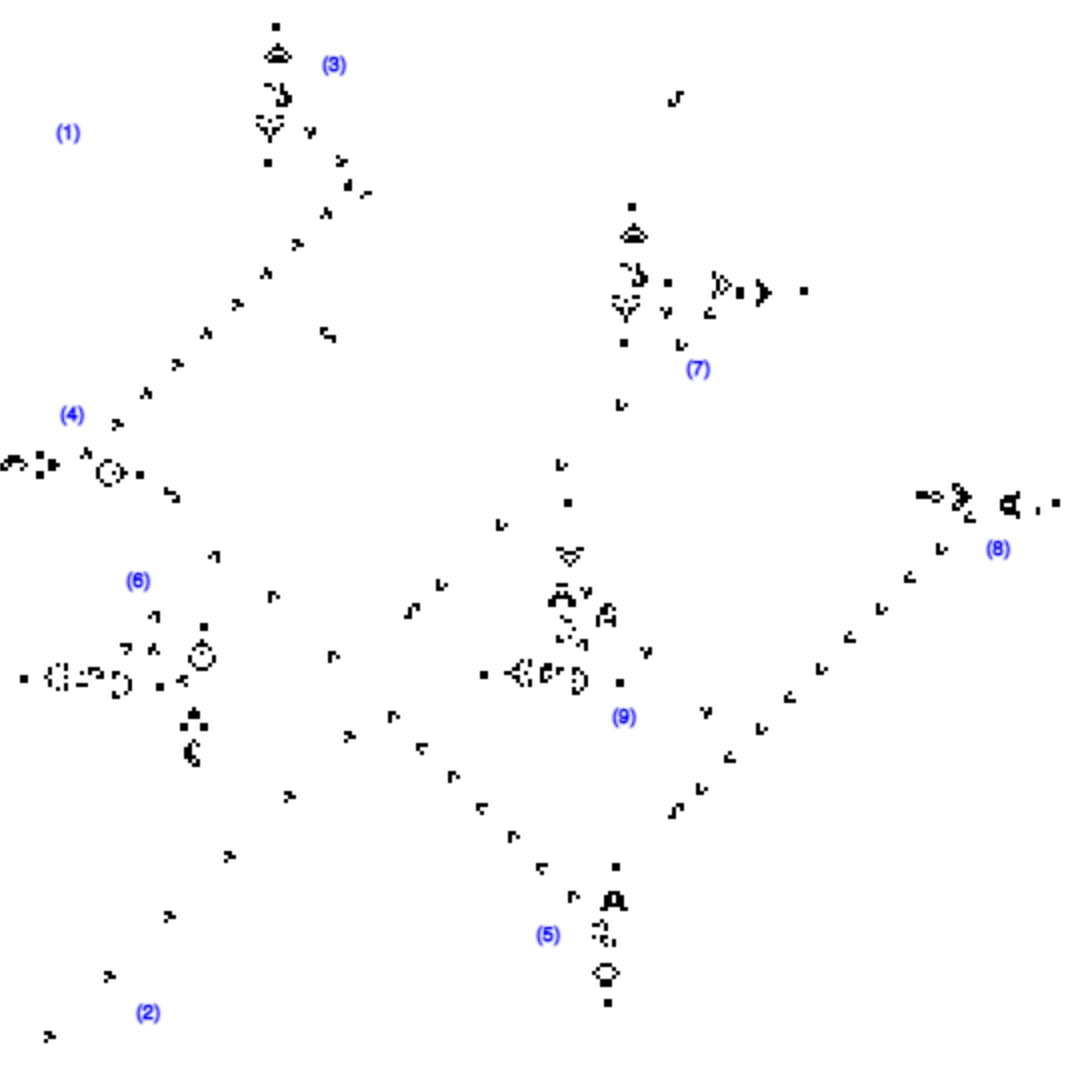
\includegraphics[width=\linewidth]{figures/andNoGo1.png} % Placeholder - Replace with actual image if available
  \end{minipage}

  \vspace{1em} % Add some vertical space between rows

  % Case 10 -> 0
  \begin{minipage}{0.45\textwidth}
    \centering
    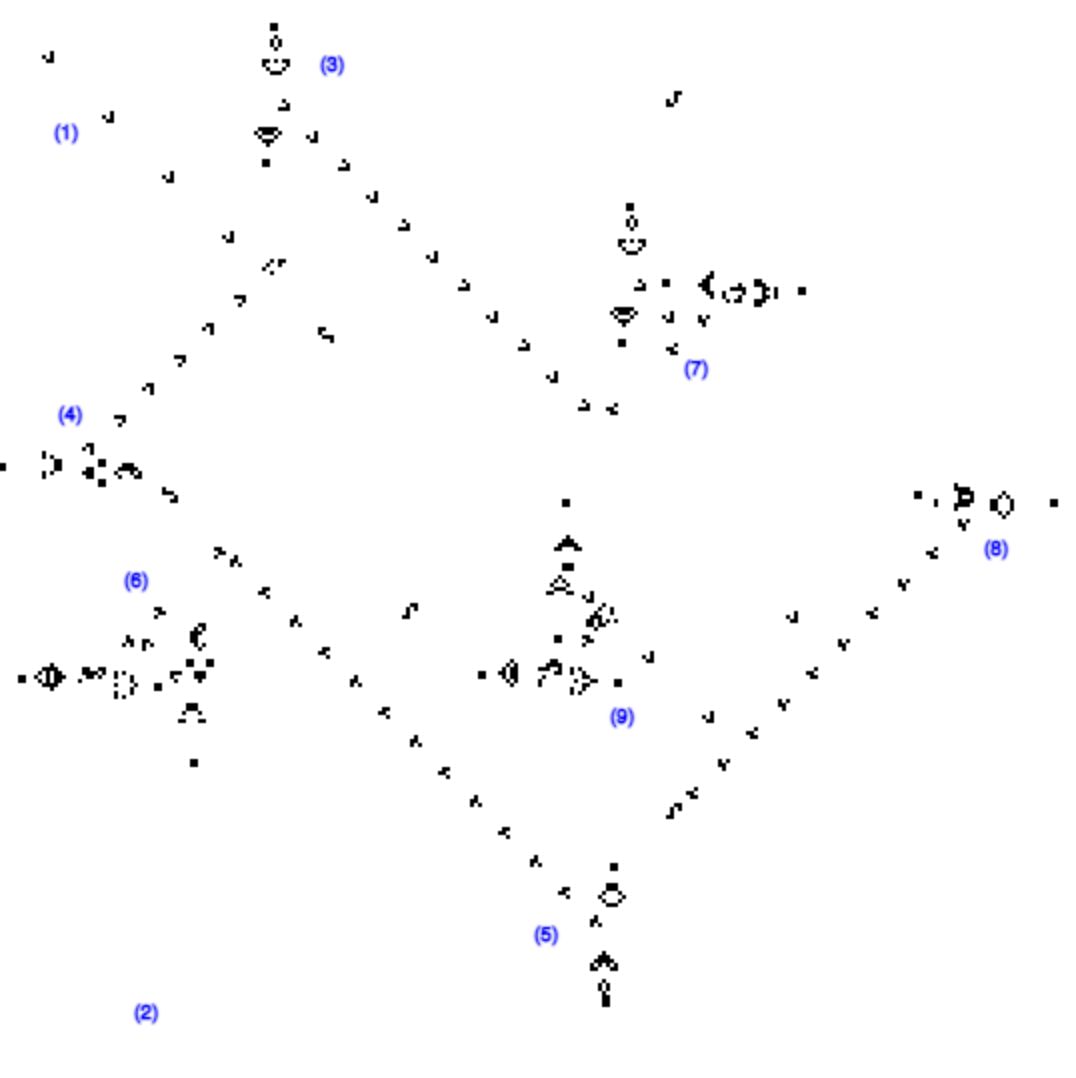
\includegraphics[width=\linewidth]{figures/andNoGo2.png} % Placeholder - Replace with actual image if available
  \end{minipage}\hfill
  % Case 11 -> 1
  \begin{minipage}{0.45\textwidth}
    \centering
    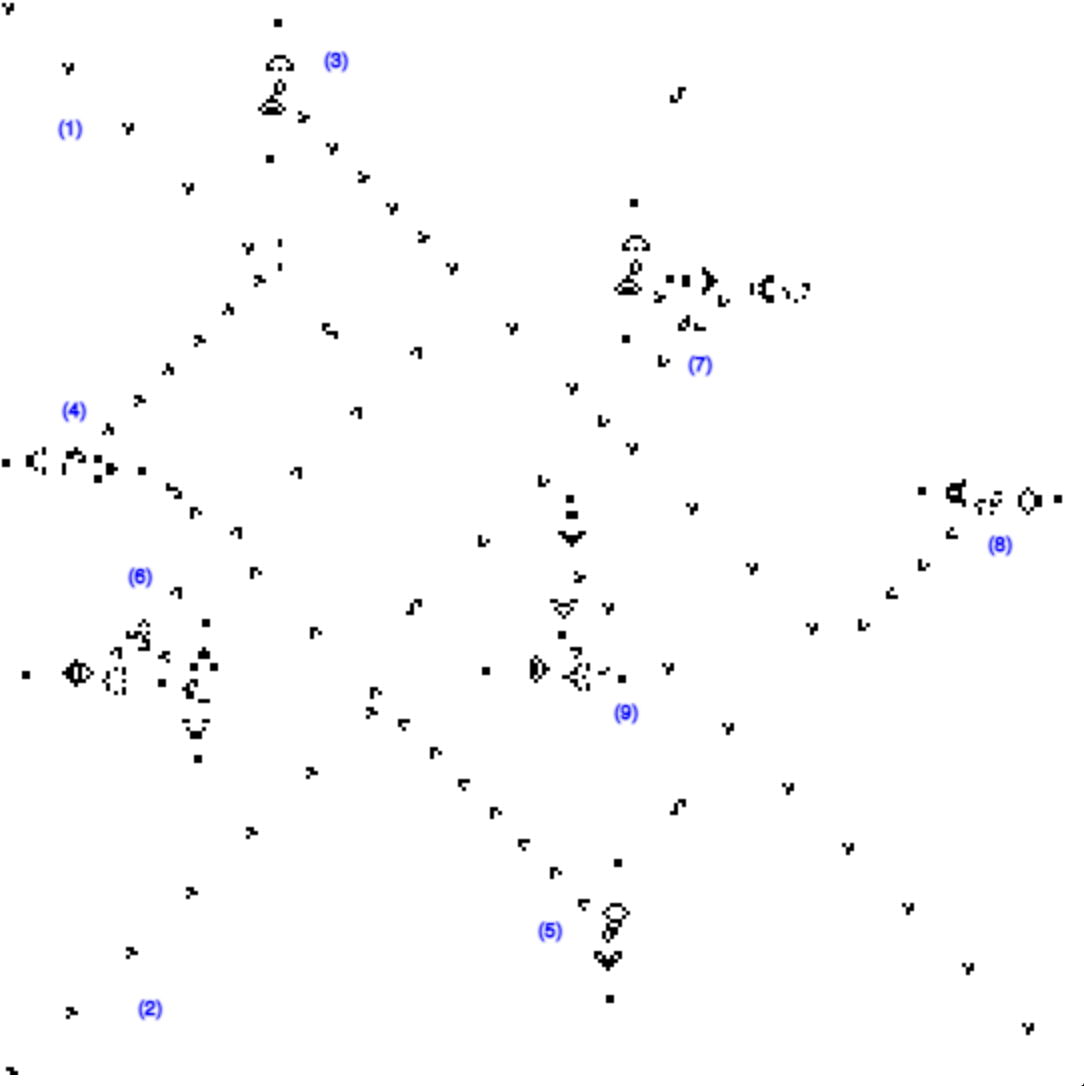
\includegraphics[width=\linewidth]{figures/andGo.png} % Placeholder - Replace with actual image if available
  \end{minipage}

  \caption{Behavior of a glider-based AND gate for inputs (1) and (2). Top Left: Input (0,0) yields Output 0. Top Right: Input (0,1) yields Output 0. Bottom Left: Input (1,0) yields Output 0. Bottom Right: Input (1,1) yields Output 1. \cite{Carlini_2020}}
  \label{fig:and-gate}
\end{figure}

\paragraph{OR Gate:} An OR gate can often be constructed by carefully merging two input streams towards the output path.
\begin{itemize}
  \item \textbf{Input ('1', '0') or ('0', '1'):} The single present glider is routed directly onto the output path $S_{out}$. Result: Output '1'.
  \item \textbf{Input ('1', '1'):} Both gliders arrive. The collision must be managed such that either only one glider survives and proceeds onto $S_{out}$, or they annihilate each other but trigger the release of a third, pre-positioned glider onto $S_{out}$. A simpler approach might involve ensuring the paths merge such that gliders arriving from either input end up on the same output track, possibly with timing adjustments needed if simultaneous arrival causes annihilation. Result: Output '1'.
  \item \textbf{Input ('0', '0'):} No gliders arrive. Result: Output '0'.
\end{itemize}
Alternatively, OR can be constructed using AND and NOT gates via De Morgan's laws: $A \lor B = \neg (\neg A \land \neg B)$.

\begin{figure}[H]
  \centering
  % Case 00 -> 0
  \begin{minipage}{0.45\textwidth}
    \centering
    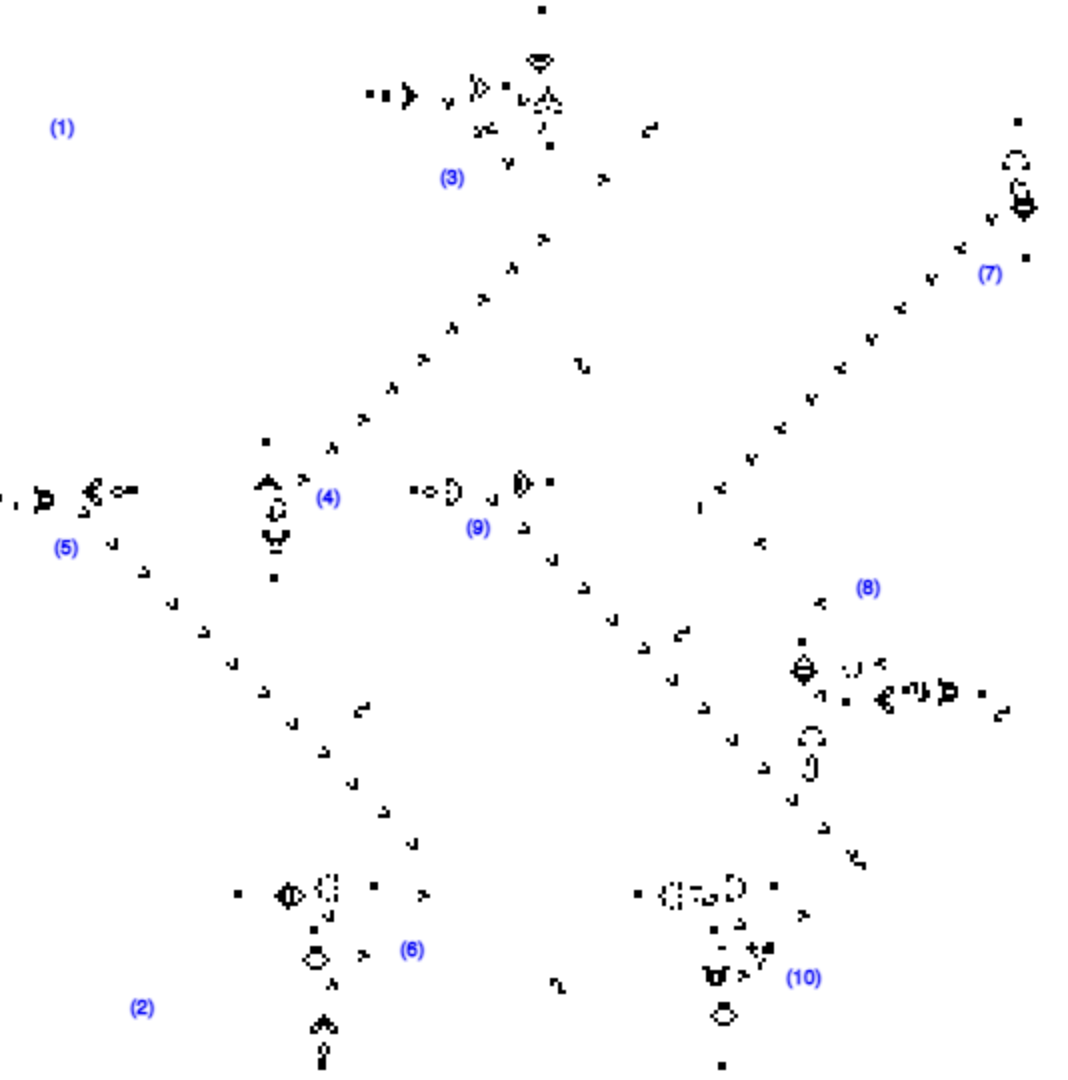
\includegraphics[width=\linewidth]{figures/orNoGo.png}
  \end{minipage}\hfill
  % Case 01 -> 1
  \begin{minipage}{0.45\textwidth}
    \centering
    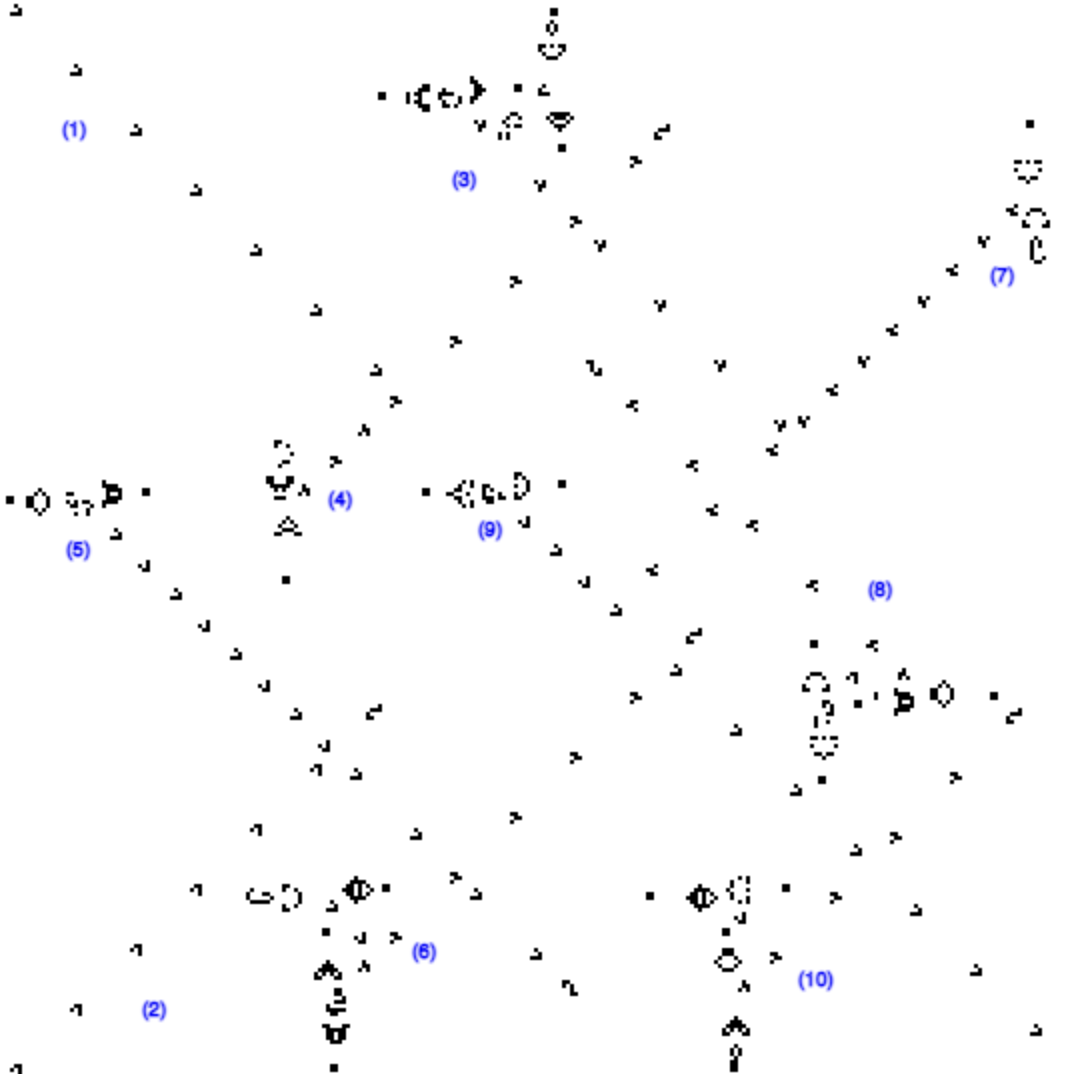
\includegraphics[width=\linewidth]{figures/orGo2.png}
  \end{minipage}

  \vspace{1em} % Add some vertical space between rows

  % Case 10 -> 1
  \begin{minipage}{0.45\textwidth}
    \centering
    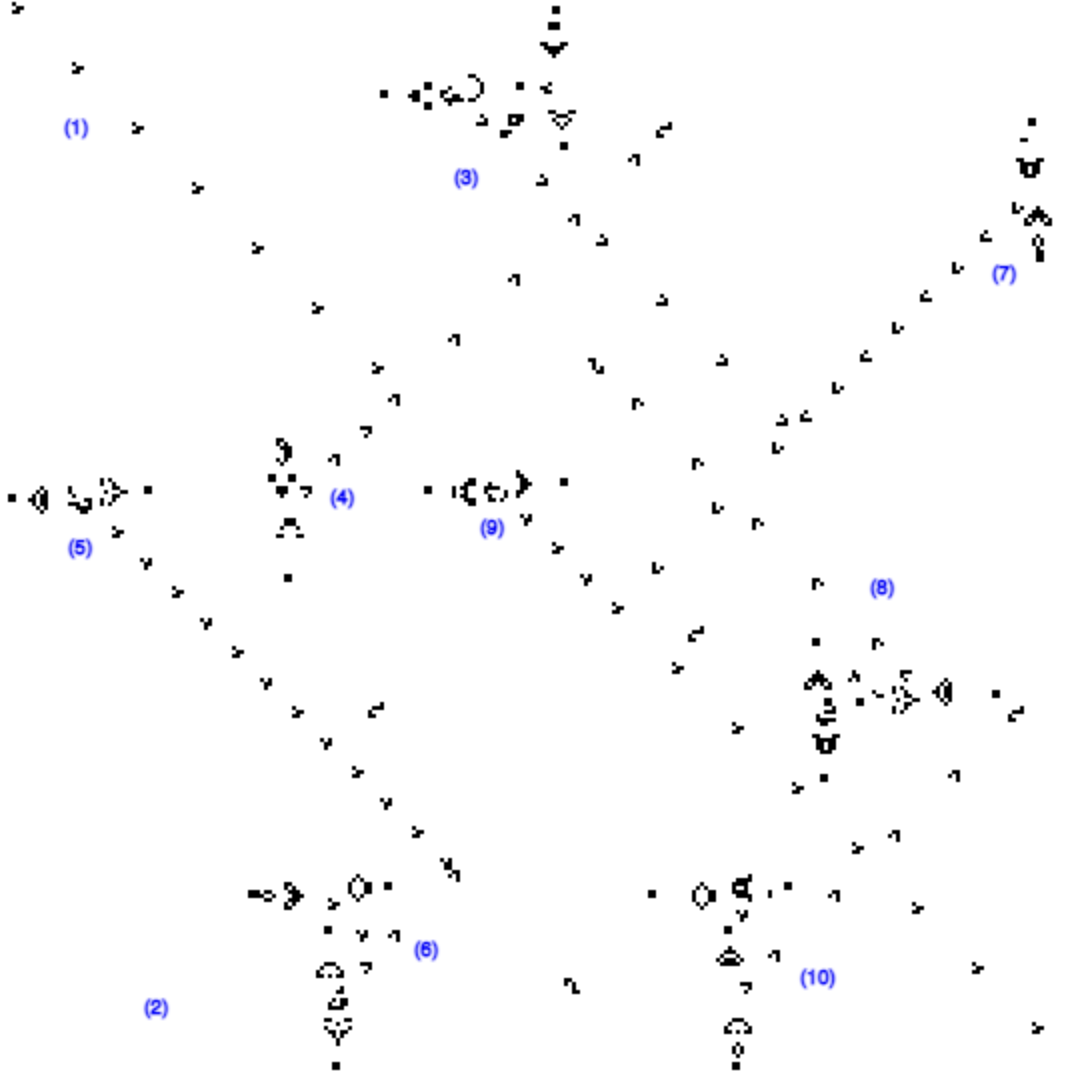
\includegraphics[width=\linewidth]{figures/orGo1.png}
  \end{minipage}\hfill

  \caption{Behavior of a glider-based OR gate for inputs (1) and (2). Top Left: Input (0,0) yields Output 0. Top Right: Input (0,1) yields Output 1. Bottom: Input (1,0) yields Output 1. \cite{Carlini_2020}}
  \label{fig:or-gate}
\end{figure}

These constructions, while conceptually simple, are practically complex, requiring large spatial arrangements and precise timing managed by carefully positioned glider guns and absorbers. The existence of such constructible gates, however, demonstrates that arbitrary Boolean logic can, in principle, be implemented within Conway's Game of Life using glider streams as signals. This forms a crucial step towards building more complex computational structures, like the components of a Turing machine. Examples of specific glider collisions achieving these effects have been cataloged and utilized in complex constructions, some of which we'll be talking about in a bit.


\subsubsection{Memory Elements and the Tape}

To simulate a Turing machine, we need not only logic gates to implement the transition function but also a way to represent the machine's tape and store information on it. In Conway's Game of Life, this is achieved by constructing patterns that can exist in (at least) two distinct stable or predictably evolving states, representing the binary symbols (typically '0' and '1') on the tape. These patterns function as memory cells.

\begin{definition}[Memory Cell in Life]
A \textit{memory cell} is a configuration $M$ in Conway's Game of Life designed such that:
\begin{enumerate}
  \item It can stably exist in at least two distinct states, $S_0$ and $S_1$, representing binary '0' and '1'. These states might be still lifes, oscillators, or even specific configurations of glider streams (e.g., presence/absence in a loop).
  \item Its state can be reliably "read" by interacting with it using specific input glider streams. Reading typically involves sending a glider that is either destroyed/deflected differently depending on the cell's state, or that triggers the emission of an output glider only if the cell is in a particular state. The read operation should ideally leave the cell's state unchanged.
  \item Its state can be reliably "written" (or flipped) by interacting with it using specific input glider streams. A 'write 0' signal should force the cell into state $S_0$, and a 'write 1' signal should force it into state $S_1$, regardless of its previous state.
\end{enumerate}
\end{definition}

Various mechanisms have been devised for memory cells:

\begin{itemize}
  \item \textbf{Stable Pattern Manipulation:} Simple still lifes like the 'block' or 'boat' can be destroyed by precisely aimed gliders. A memory cell could consist of the presence (state '1') or absence (state '0') of such a still life at a specific location. Writing '1' involves a glider collision that creates the still life, while writing '0' involves a collision that destroys it. Reading might involve sending a glider along a path that is blocked only if the still life is present.
  \item \textbf{Oscillator Manipulation:} Certain oscillators can be perturbed by gliders to shift their phase or change their form into another stable oscillator or still life. For example, an oscillator might be "toggled" between two phases or states by successive glider impacts.
  \item \textbf{Glider Loops:} A more dynamic approach involves using circulating loops of gliders. The presence or absence of a glider in the loop at a specific point in its cycle can represent '1' or '0'. Gliders can be injected into or ejected from the loop via carefully timed collisions at specific junctions.
\end{itemize}

To simulate the Turing machine's tape, these individual memory cells are arranged linearly across the Life grid.

\begin{definition}[Tape Representation in Life]
A Turing machine tape is represented as a linear array of memory cells $(M_i)_{i \in \mathbb{Z}}$ positioned along a line (or path) in the Life grid. The state of cell $M_i$ corresponds to the symbol stored in the $i$-th cell of the simulated TM tape.
\end{definition}

The infinite nature of the Life grid naturally accommodates the concept of an infinite TM tape. While any specific construction will be finite, mechanisms can be designed to extend the tape representation dynamically if the simulated TM head moves beyond the currently constructed portion. This often involves "tape constructor" units that lay down new memory cells (typically initialized to a 'blank' state) as needed.

The interaction between the TM's read/write head (simulated by glider streams and logic circuits) and the tape involves directing gliders to the specific memory cell corresponding to the head's current position. Gliders are sent to read the cell's state, the information is processed by the logic gate circuitry (simulating the TM's transition function), and then further gliders are sent to write the new symbol to the cell and trigger the simulated movement of the head (typically by activating logic that targets the next cell to the left or right).

Constructing reliable, densely packed, and easily addressable memory cells is a significant engineering challenge within Life, but feasible designs exists. They are far too complex to convey in full here

\subsubsection{Simulating the Read/Write Head and State Control}

The final crucial components for simulating a Turing machine in Conway's Game of Life are the mechanisms that represent the TM's finite state control and its read/write head. These elements must interact with the tape representation (memory cells) and the logic circuits (transition function implementation) to orchestrate the computation step-by-step.

\begin{definition}[State Representation in Life]
The internal state of the simulated Turing machine (from its finite set of states $Q$) is typically represented by a dedicated set of memory cells or a specific configuration of active patterns (e.g., circulating gliders) within a designated "control unit" region of the Life grid. If there are $|Q|$ states, $\lceil \log_2 |Q| \rceil$ binary memory cells are sufficient to encode the current state.
\end{definition}

\begin{definition}[Read/Write Head Simulation]
The read/write head's position and actions are simulated through precisely controlled glider streams and logic:
\begin{enumerate}
  \item \textbf{Position:} The head's current position over the tape (which memory cell $M_i$ is being accessed) is not usually represented by a physical marker moving along the tape. Instead, it's implicitly encoded by which memory cell the control circuitry is currently interacting with. Logic circuits direct the read/write glider streams to the target cell $M_i$.
  \item \textbf{Reading:} To read the symbol at the current head position $i$, the control unit sends a "read" glider signal towards memory cell $M_i$. The interaction of this glider with $M_i$ produces an output signal (e.g., another glider or its absence) that travels back to the control unit, indicating the symbol ('0' or '1') stored in $M_i$.
  \item \textbf{State Transition Logic:} The read symbol signal, along with the signals representing the current state (read from the state memory cells), are fed as inputs to the logic gate network that implements the TM's transition function $\delta(q, \gamma)$.
  \item \textbf{Writing:} Based on the output of the transition function logic, which specifies the new symbol $\gamma'$ to be written, the control unit sends a corresponding "write" glider signal (e.g., 'write 0' or 'write 1') to the current memory cell $M_i$. This signal interacts with $M_i$ to set its state to $\gamma'$.
  \item \textbf{Moving:} The transition function output also specifies the head movement (Left, Right, or Stay). The control logic interprets this output and updates its internal targeting mechanism to interact with the next appropriate memory cell ($M_{i-1}$ or $M_{i+1}$) in the subsequent cycle. This might involve activating different glider paths or adjusting timing sequences.
  \item \textbf{State Update:} Finally, the transition function output specifies the next state $q'$. The control unit sends signals to update the state memory cells to reflect this new state $q'$.
\end{enumerate}
\end{definition}

This entire process constitutes one step of the simulated Turing machine. It involves a complex sequence of timed glider emissions, collisions, and signal propagations between the control unit, the logic gates, and the targeted memory cell on the tape. The control unit acts as the central orchestrator, managing the timing and routing of glider streams based on the current state and the symbol read from the tape.

Constructing this control circuitry is arguably the most complex part of building a TM in Life. It requires integrating the logic gates and memory cell interaction mechanisms into a cohesive system that correctly sequences the read, transition, write, move, and state update operations according to the specific TM being simulated. Again, it's outside of the scope of this writeup to detail in full, but it should be believable that, with proper synchronization, things fall into place here.


\subsubsection{Integration and Overall Architecture}

The construction of a functional Turing machine within Conway's Game of Life requires the meticulous integration of the previously described components: glider-based logic gates, memory cell arrays representing the tape, and the control circuitry simulating the finite state automaton and read/write head operations. This integration forms a single, vast, and intricate pattern on the Life grid whose evolution over discrete generations precisely mirrors the computational steps of the target Turing machine.

\paragraph{Spatial Layout and Connectivity:}
The overall architecture necessitates a carefully planned spatial layout on the infinite grid to prevent unwanted interference between components. Key areas include:
\begin{enumerate}
  \item \textbf{Control Unit Region:} A dedicated area housing the logic gates that implement the TM's transition function ($\delta$) and the memory elements storing the TM's current state ($q \in Q$).
  \item \textbf{Tape Region:} A (conceptually infinite) linear arrangement of memory cells ($M_i$), typically extending horizontally or vertically. Each cell $M_i$ stores one tape symbol ($\gamma$).
  \item \textbf{Glider Pathways:} A network of precisely defined paths connecting the control unit to the tape cells and interconnecting logic gates within the control unit. These paths guide the glider streams carrying information (read requests, read data, write commands, state information, clock signals). Path routing must ensure gliders arrive at their destinations without colliding unintentionally with other streams or static components. "Glider reflectors" or specific collision outcomes might be used to turn streams 90 or 180 degrees.
  \item \textbf{Signal Generation and Termination:} Glider guns are strategically placed to generate the necessary clock signals and data-carrying gliders. Glider "eaters" (stable patterns that absorb gliders without generating debris) are positioned at the end of pathways or where signals need to be terminated cleanly.
\end{enumerate}
Sufficient empty space must separate these regions and pathways to maintain signal integrity.

\paragraph{Temporal Synchronization and Clocking:}
The simulation operates in discrete cycles, each corresponding to one step of the Turing machine. Temporal synchronization is paramount and typically achieved through:
\begin{enumerate}
  \item \textbf{Master Clock:} One or more synchronized glider guns emitting periodic "clock" gliders. These pulses trigger sequential phases within a single TM step (e.g., initiate read, trigger logic evaluation, initiate write, trigger move/state update).
  \item \textbf{Path Length Engineering:} The time taken for a glider to travel between components is determined by the path length. Designers meticulously calculate these lengths to ensure signals arrive in the correct sequence and with the necessary delays for processing at each stage. For instance, the signal representing the read symbol must arrive at the transition function logic simultaneously with the signal representing the current state.
\end{enumerate}

\paragraph{Operational Cycle (Simulating one TM step $\delta(q, \gamma) = (q', \gamma', D)$):}
A typical cycle proceeds as follows:
\begin{enumerate}
  \item \textbf{Initiation (Clock Pulse 1):} The control unit, using its internal representation of the current head position $i$, sends a "read" glider stream towards memory cell $M_i$. Simultaneously, the current state $q$ is read from the state memory within the control unit.
  \item \textbf{Read Propagation:} The read glider interacts with $M_i$. The outcome (e.g., a reflected glider, a newly generated glider, or absence thereof) representing the tape symbol $\gamma$ travels back along a designated path to the control unit's transition logic inputs.
  \item \textbf{Logic Evaluation (Clock Pulse 2):} The $\gamma$ signal and the $q$ signal arrive at the inputs of the logic gate network implementing $\delta$. The network computes the outputs: the next state $q'$, the symbol to write $\gamma'$, and the direction to move $D \in \{L, R, S\}$.
  \item \textbf{Write Operation (Clock Pulse 3):} Based on the computed $\gamma'$, the control unit sends the appropriate "write $\gamma'$" glider stream to memory cell $M_i$, updating its state.
  \item \textbf{State Update and Move Preparation (Clock Pulse 4):} The control unit updates its internal state memory to $q'$. Based on the computed direction $D$, it adjusts its internal addressing mechanism to target cell $M_{i-1}$ (if $D=L$) or $M_{i+1}$ (if $D=R$) for the next cycle. This might involve enabling different glider guns or redirecting pathways for the next read signal.
\end{enumerate}
This sequence ensures that each TM step is faithfully executed through coordinated glider interactions within the Life pattern.

\paragraph{Initialization and Execution:}
To run a specific computation, the Life grid must be initialized with the pattern representing the TM construction, along with the initial configuration: the starting state $q_0$ encoded in the control unit, the input string encoded on the tape cells (with others typically set to the blank symbol), and the initial head position set in the control unit's targeting logic. The simulation then proceeds autonomously according to the rules of Life, with the pattern's evolution directly corresponding to the TM's computation.

\begin{figure}[H]
  \centering
  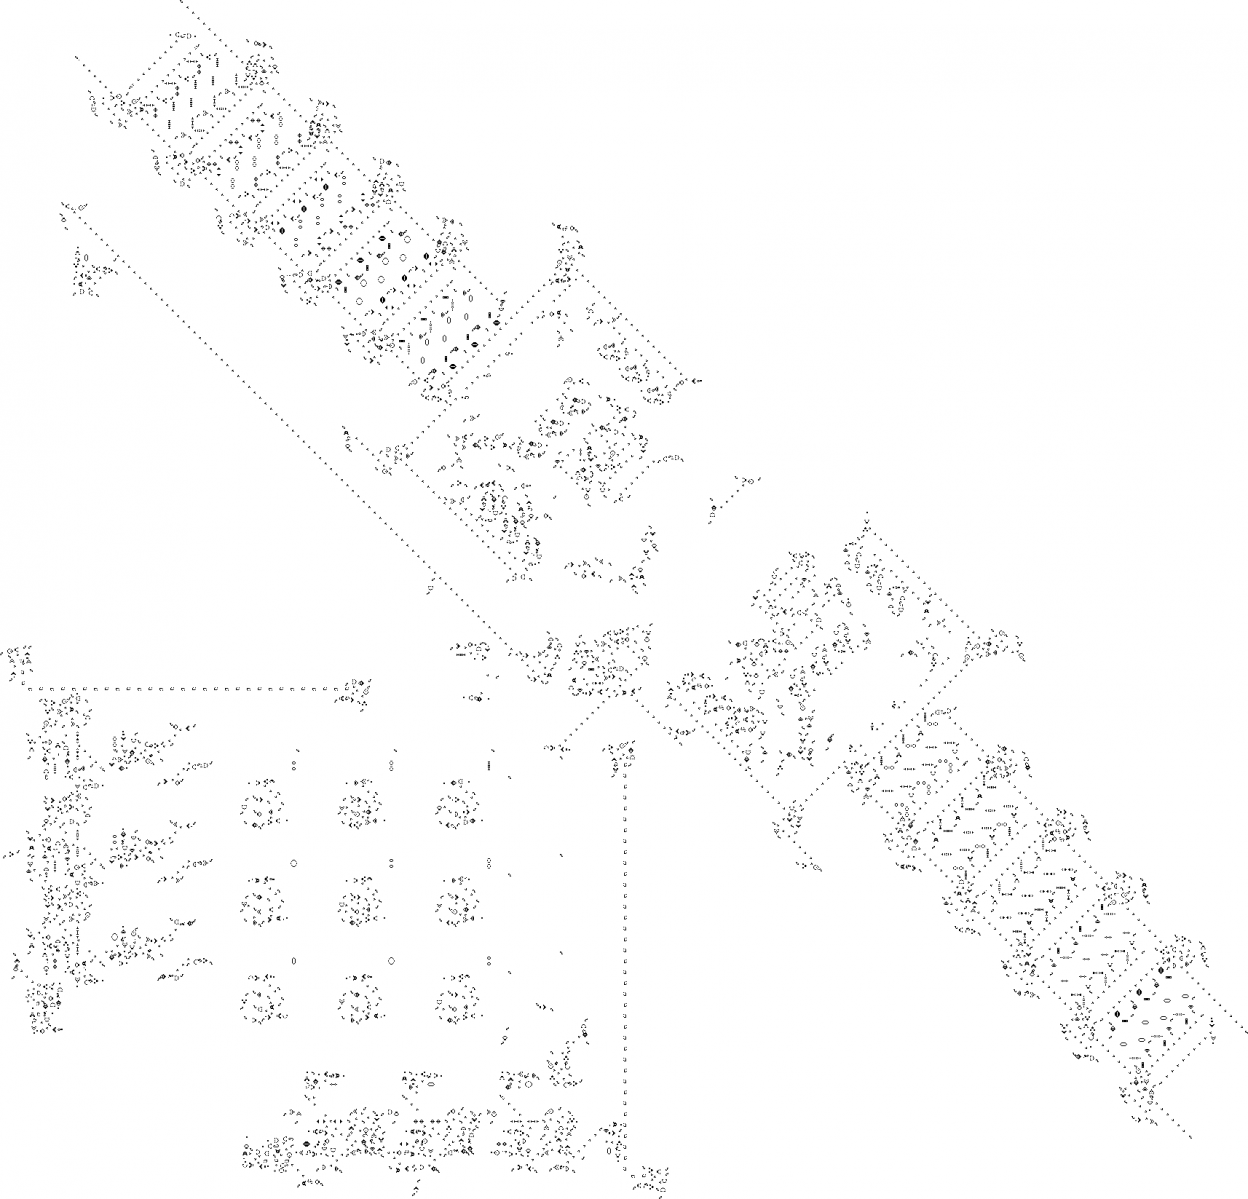
\includegraphics[width=0.8\textwidth]{figures/TM.png} % Placeholder for actual UTM image
   \caption{A TM in Life \cite{Rendell_2005_TM}}
  \label{fig:utm-in-life}
\end{figure}

So, we can construct a TM in Life. What's next?

\subsection{Constructing a Universal Constructor \cite{Burks_1970_Essays}} 
While the previous sections established that complex computations, akin to those performed by specific Turing machines, can be implemented in Conway's Game of Life, John von Neumann's original explorations into cellular automata were motivated by an even more profound question related to the logic of life: Can a machine construct any other machine described to it, including a copy of itself? This led to the concept of a \textit{Universal Constructor} (UC).

The idea of universality is key here. Just as we will soon discuss the \textit{Universal Turing Machine} (UTM) – a machine capable of simulating any other Turing machine – the UC represents a similar universality but in the domain of construction. A UC is envisioned as a machine that, given a description or "blueprint," can build the described machine within the cellular automaton grid. If the blueprint describes the UC itself, it achieves self-replication.

The significance of demonstrating that a UC can be built within Conway's Game of Life is profound. It would show not only computational power (as the UC needs to process the blueprint, likely requiring UTM-like capabilities which we will detail shortly) but also \textit{constructional universality} and the capacity for self-replication—properties often considered fundamental characteristics of living systems. While the UTM concept (to be defined next) focuses on simulating any computation, the UC concept focuses on simulating any construction, including its own. Achieving this within Life would provide a powerful argument for its ability to model complex, life-like behaviors involving both computation and physical reproduction.

\subsubsection{Von Neumann's Universal Constructor Concept}
John von Neumann conceptualized a \textit{Universal Constructor} (UC) as a theoretical machine operating within a cellular automaton environment, capable of constructing any machine specified by a description, including itself. Formally, a UC can be defined by its essential components and capabilities:

\begin{enumerate}
  \item \textbf{Blueprint (Description Tape):} A one-dimensional sequence of states or symbols encoded on a structure within the cellular automaton (analogous to a TM tape). This blueprint contains the complete description $\mathcal{D}(M)$ of the machine $M$ to be constructed. For self-replication, the blueprint would be $\mathcal{D}(\text{UC})$.

  \item \textbf{Universal Constructor Proper (Construction Unit):} The core mechanism responsible for manipulating the cellular automaton grid. It reads instructions from the blueprint and executes them by changing the states of cells in a designated construction area. This involves:
    \begin{itemize}
      \item A \textit{construction arm} capable of moving within the grid and modifying cell states at specific locations (e.g., setting a cell to 'live' or 'dead' in Life).
      \item Mechanisms to fetch raw materials (e.g., quiescent cells) or manage the construction process.
    \end{itemize}

  \item \textbf{Universal Computer (Controller):} An embedded computational device, functionally equivalent to a Universal Turing Machine (UTM). Its role is to:
    \begin{itemize}
      \item Read and interpret the instructions encoded on the blueprint tape.
      \item Coordinate and control the actions of the construction unit based on the interpreted instructions.
      \item Manage internal state and logic required for the construction process.
    \end{itemize}

  \item \textbf{Blueprint Copying Mechanism:} A crucial component, often integrated with the controller and constructor, capable of accurately duplicating the blueprint tape. This is essential for self-replication, ensuring the newly constructed machine also possesses the blueprint.
\end{enumerate}

The primary goal of the UC concept was to demonstrate rigorously that machines could exist within a formal system (like a cellular automaton) that are capable of \textit{non-trivial self-replication}. This involves constructing a copy of themselves that possesses the same complexity and capabilities, including the ability to construct further copies. Von Neumann's work aimed to show that reproduction of complexity equal to or greater than the parent machine was logically possible, providing foundational insights into theoretical biology and artificial life. The existence of a UC within a system like Conway's Game of Life implies not only Turing completeness (due to the embedded universal computer) but also constructional universality and the potential for complex self-organization and replication.

\subsubsection{Requirements for a UC in Conway's Game of Life}
To realize von Neumann's concept of a Universal Constructor within the framework of Conway's Game of Life, a pattern must embody a specific set of sophisticated functional capabilities. These capabilities, implemented through intricate arrangements of interacting Life structures (like gliders, logic gates, and memory elements), must collectively enable the pattern to interpret a description and build the corresponding machine, potentially including itself. The essential requirements are:

\begin{enumerate}
  \item \textbf{Blueprint Storage:} The pattern must incorporate a mechanism capable of storing the blueprint, $\mathcal{D}(M)$, which is the complete description of the machine $M$ to be constructed. This storage medium would likely be analogous to the Turing machine tape discussed previously, implemented as a linear array of memory cells capable of holding the encoded instructions.

  \item \textbf{Blueprint Interpretation:} A computational component, functionally equivalent to a Universal Turing Machine or a sufficiently powerful logic circuit built from glider-based gates, must be present. This component is responsible for reading the blueprint from the storage medium, parsing the instructions, and translating them into control signals for the construction mechanism.

  \item \textbf{Environmental Manipulation (Construction Arm):} The pattern must possess the ability to modify the state of cells in the surrounding Game of Life grid in a controlled manner. This function, often conceptualized as a "construction arm," would likely be implemented using precisely directed streams of gliders or other engineered patterns. These streams must be capable of creating specific basic structures (e.g., placing live cells, forming blocks or blinkers) or erasing existing ones at designated coordinates in the construction area, effectively "printing" the target machine onto the grid.

  \item \textbf{Coordination and Control:} A central control unit (integrated within the computational component) is required to orchestrate the entire process. It must sequence the operations: fetching instructions from the blueprint, interpreting them, directing the construction arm, managing internal states, and potentially handling error conditions or resource management (e.g., ensuring clear space for construction).

  \item \textbf{Blueprint Copying:} For true self-replication (where the constructed machine is also a UC), the pattern must include a mechanism to accurately duplicate its own blueprint, instruction by instruction, and transfer this copy to the storage medium of the newly constructed machine. This ensures the offspring possesses the necessary information to replicate further.

  \item \textbf{Structural Replication:} Ultimately, the integrated system must be capable of constructing a complete and functional copy of the entire Universal Constructor pattern itself—including its blueprint storage, interpretation logic, control unit, construction arm, and copying mechanism.
\end{enumerate}

Meeting these requirements within the simple rules of Conway's Game of Life necessitates patterns of extraordinary complexity and size, far exceeding those typically observed in casual explorations of the game. However, the theoretical possibility of constructing such patterns underscores the profound computational and constructional depth inherent in Life.

\subsubsection{Implementing Construction Mechanisms: The Construction Arm}
The realization of a Universal Constructor within Conway's Game of Life hinges on the ability to physically manipulate the grid environment according to blueprint specifications. This manipulation is performed by a conceptual component known as the \textit{construction arm}. Formally, the construction arm is not a single monolithic pattern but rather a complex subsystem within the UC pattern designed to emit precisely controlled sequences of mobile patterns (primarily gliders) that interact at designated target coordinates in the grid to modify cell states.

\begin{definition}[Construction Arm Functionality]
Let $G_{UC}$ be the pattern representing the Universal Constructor. The construction arm subsystem $A \subseteq G_{UC}$ provides the following capabilities:
\begin{enumerate}
  \item \textbf{Targeting:} Based on coordinate information $(x, y)$ derived from the blueprint instructions and processed by the UC's control unit, $A$ can generate and direct output patterns towards the cell at $(x, y)$.
  \item \textbf{State Modification:} The emitted patterns are engineered such that their interaction at or near $(x, y)$ results in a predictable change in the state of the cell at $(x, y)$ and potentially its immediate neighbors. This includes:
    \begin{itemize}
      \item \textbf{Cell Creation (Setting State to 'Live'):} Emitting specific glider sequences whose collision at $(x, y)$ synthesizes a live cell, potentially as part of a larger basic pattern (e.g., a block). This requires collisions that leave behind the desired residue. For example, specific head-on or angled glider collisions are known to produce stable or simple oscillating patterns.
      \item \textbf{Cell Deletion (Setting State to 'Dead'):} Emitting glider sequences whose collision at $(x, y)$ annihilates any existing live cell(s) at that location without leaving persistent debris, or interacts with a specific known pattern to remove it cleanly. This often involves using gliders to perturb a pattern into an unstable configuration that quickly dies out, or employing patterns known as "eaters" which consume specific incoming patterns.
    \end{itemize}
  \item \textbf{Precision and Non-interference:} The targeting and state modification must be sufficiently precise to affect only the intended location and avoid disrupting the UC pattern itself or previously constructed parts of the target machine. This necessitates careful path planning for the construction gliders and potentially the use of "scaffolding" or temporary patterns that are later removed.
\end{enumerate}
\end{definition}

The implementation relies heavily on the principles of glider synthesis and interaction discussed earlier. The UC's internal logic (the embedded UTM) translates blueprint commands like "Place block at (x,y)" or "Clear cell at (x,y)" into sequences of activation signals for specific glider guns within the construction arm subsystem. These guns then emit the required gliders along pre-defined pathways. The geometry of these pathways and the timing of glider emissions are critical. Techniques such as using glider reflectors (patterns that change a glider's trajectory) allow the arm to reach various locations from a fixed set of emitters.

Construction typically proceeds by assembling the target machine from a predefined set of basic, constructible building blocks (e.g., blocks, blinkers, specific glider syntheses) rather than placing every single live cell individually. The blueprint encodes instructions for placing these blocks. The construction arm, therefore, needs to be capable of synthesizing these fundamental patterns reliably at arbitrary specified locations within the construction zone. The complexity lies in orchestrating these emissions and ensuring that the construction gliders arrive correctly and interact as intended, often requiring intricate timing managed by the UC's internal clock mechanisms. The existence of known glider collisions that can synthesize basic stable patterns and others that can cleanly remove them provides the foundation for this capability.

\subsubsection{Encoding the Blueprint and the Replication Process}
For a Universal Constructor (UC) to function, particularly for self-replication, the description of the machine to be built—the blueprint—must be encoded in a format that the UC can read and process. Within Conway's Game of Life, this blueprint is typically stored on a linear structure analogous to a Turing machine tape, composed of the memory cells previously discussed.

\begin{definition}[Blueprint Encoding]
Let $M$ be the machine to be constructed by the UC. The \textit{blueprint} $\mathcal{D}(M)$ is a finite sequence of symbols from a predefined alphabet $\Sigma_{blueprint}$. This sequence encodes the complete structural and functional specification of $M$, including the types and relative positions of all necessary components (e.g., logic gates, memory cells, glider guns, pathways) and their initial states. The encoding scheme must be such that the UC's internal computational unit (its embedded UTM) can parse $\mathcal{D}(M)$ and translate it into a sequence of elementary construction actions (e.g., "place block at relative coordinate $(x,y)$," "emit glider type $G$ towards target $T$"). The blueprint $\mathcal{D}(M)$ is physically represented on the Life grid as the sequence of states ($S_0$ or $S_1$) of an array of memory cells $(B_j)_{j=1}^{|\mathcal{D}(M)|}$ integrated within the UC pattern. For self-replication, the blueprint is $\mathcal{D}(\text{UC})$.
\end{definition}

The process of self-replication, where a UC constructs a copy of itself, involves a carefully orchestrated sequence of operations managed by the UC's control unit:

\begin{enumerate}
  \item \textbf{Blueprint Reading:} The UC begins by accessing its own blueprint tape, $\mathcal{D}(\text{UC})$, stored within its structure. Its internal UTM reads the instructions sequentially.
  \item \textbf{Instruction Interpretation:} Each instruction read from the blueprint is processed by the UC's computational logic. This logic determines the necessary actions for the construction arm (e.g., target coordinates, type of pattern to synthesize or erase).
  \item \textbf{Construction Execution:} The control unit directs the construction arm subsystem. Based on the interpreted instructions, the arm emits precisely timed and aimed glider sequences to build a new, identical UC structure in an adjacent clear area of the grid. This involves assembling the necessary components piece by piece according to the blueprint.
  \item \textbf{Blueprint Copying:} This is a critical and complex phase. As the new UC structure is being built (or after its basic framework is complete), the parent UC must duplicate its entire blueprint, $\mathcal{D}(\text{UC})$, instruction by instruction. This involves reading each symbol from its own blueprint tape and using the construction arm (or a specialized copying mechanism) to write that symbol onto the corresponding memory cell of the new UC's blueprint tape. This ensures the offspring inherits the complete instructions for further replication.
  \item \textbf{Activation:} Once the new UC structure is fully assembled and its blueprint tape is completely copied, the parent UC may send a final activation signal (e.g., a specific glider pattern) to initiate the operation of the newly constructed UC. The offspring is now capable of independent operation and replication.
\end{enumerate}

The realization of such a process within Conway's Game of Life represents a monumental feat of cellular automaton engineering. The patterns required are extraordinarily large and complex, involving potentially billions of live cells arranged with intricate precision. While a complete, running self-replicating pattern based on von Neumann's full UC concept has been theoretically designed and partially simulated (e.g., Renato Nobili's and Tim Hutton's work on self-replicating loops which simplify the construction task, or Paul Rendell's work on TM components), constructing and running a full UC in Life pushes the boundaries of computational resources. Nevertheless, the theoretical demonstration that such constructions are possible, building upon the Turing completeness and the existence of constructible logic gates, memory, and controlled glider manipulation, solidifies the status of Conway's Game of Life as a system capable of both universal computation and universal construction, including self-replication.


\subsection{Constructing a Universal Turing Machine \cite{Goucher_2011_UTM}}
% Outline for Section: Constructing a Universal Turing Machine

% This section builds upon the previous discussions of simulating specific TMs 
% and the concept of universal construction. It focuses specifically on the 
% construction of a Universal Turing Machine (UTM) within Conway's Game of Life.
% The goal is to explain what a UTM is, how its components (which are more 
% complex than a standard TM's) can be realized in Life, and the profound 
% implications this has, solidifying the argument for Life's Turing completeness.
% We will also touch upon the relationship between a UTM and a Universal Constructor.
Having established that specific Turing machines and even the complex mechanisms for universal construction can be conceptualized within Conway's Game of Life, we now turn to a pivotal concept: the Universal Turing Machine (UTM). This section will define the UTM – a machine capable of simulating any other Turing machine – and detail how its intricate components can be engineered using Life's patterns, particularly glider streams, logic gates, and memory. Constructing a UTM within Life is the ultimate demonstration of the game's Turing completeness, signifying its capacity for any algorithmic computation. We will also highlight the UTM's essential role as the computational core required for the functionality of a Universal Constructor.

\subsubsection{Definition of a Universal Turing Machine (UTM)}
A Universal Turing Machine (UTM), denoted as $U$, is a specific type of Turing machine with the remarkable capability to simulate the behavior of any other arbitrary Turing machine $M$. The concept formalizes the notion of a general-purpose programmable computer.

\begin{definition}[Universal Turing Machine (UTM)]
A Turing machine $U$ is a \textit{Universal Turing Machine} if, given the description $\langle M \rangle$ of an arbitrary Turing machine $M$ and an input string $w$ for $M$, $U$ can simulate the computation of $M$ on input $w$. Formally:
\begin{enumerate}
  \item \textbf{Input Format:} The input to $U$ is typically provided in a combined format, often represented as $\langle M \rangle \# w$, where $\langle M \rangle$ is a standardized encoding of the states, tape alphabet, transition function ($\delta_M$), initial state, and accepting/rejecting states of $M$, and $w$ is the input string intended for $M$. The symbol $\#$ acts as a delimiter.
  \item \textbf{Simulation Fidelity:} $U$ simulates $M$ step-by-step. The configuration of $U$ at any point reflects the corresponding configuration of $M$ (its state, tape contents, and head position).
  \item \textbf{Output Equivalence:} The behavior of $U$ on input $\langle M \rangle \# w$ mirrors the behavior of $M$ on input $w$:
    \begin{itemize}
      \item $U$ halts and accepts $\langle M \rangle \# w$ if and only if $M$ halts and accepts $w$.
      \item $U$ halts and rejects $\langle M \rangle \# w$ if and only if $M$ halts and rejects $w$.
      \item $U$ loops (runs forever) on $\langle M \rangle \# w$ if and only if $M$ loops on $w$.
    \end{itemize}
\end{enumerate}
\end{definition}

The crucial aspect of a UTM is its \textit{universality}: a single, fixed machine $U$ possesses the computational power equivalent to the entire class of Turing machines. It embodies the idea that any algorithmic procedure can be executed by this one universal device, provided the procedure itself (as TM $M$) and its input ($w$) are supplied to it in the correct format.

The existence of UTMs is a cornerstone of computability theory. It demonstrates that there are universal algorithms capable of executing any other algorithm. This theoretical foundation underpins the concept of stored-program computers, where software (the description $\langle M \rangle$) directs the operation of fixed hardware (the UTM $U$) on variable data ($w$). The construction of a UTM within Conway's Game of Life, as detailed in the subsequent sections, is the standard method for proving the game's Turing completeness.

\subsubsection{Building a UTM in Life: Integrating Components}
Constructing a Universal Turing Machine (UTM) within Conway's Game of Life builds upon the techniques used for simulating specific Turing machines, but introduces significant additional complexity due to the need to interpret an arbitrary machine description. As established previously, simulating a specific TM requires patterns implementing logic gates (for the fixed transition function), memory cells (for the tape), state control logic, and mechanisms for simulating read/write head actions using glider streams. Building a UTM necessitates enhancing and integrating these components to handle the universality requirement.

\paragraph{Enhanced Requirements for Universality:}
A UTM, $U$, must simulate any given TM, $M$, operating on input $w$. This fundamentally differs from a specific TM simulation in two key ways:

\begin{enumerate}
  \item \textbf{Multiple Tape Representations:} The UTM $U$ needs to manage information corresponding to two distinct conceptual tapes:
    \begin{itemize}
      \item \textbf{The Description Tape ($\langle M \rangle$):} This tape holds the encoded description of the machine $M$ being simulated. It contains $M$'s states, alphabet, transition function rules ($\delta_M$), initial state, etc. This tape is read-only for the UTM's control logic during the simulation phase.
      \item \textbf{The Simulated Work Tape ($w$):} This tape represents the tape of the machine $M$. The UTM must read from and write to this tape according to the rules specified in $\langle M \rangle$.
    \end{itemize}
    In a Life implementation, these could be realized as two separate linear arrays of memory cells, or potentially as distinct, marked-off sections within a single larger array.

  \item \textbf{Interpretive Control Logic:} Unlike a specific TM where the transition function $\delta$ is hardwired into the logic gate configuration, the UTM's control logic must be significantly more sophisticated. Its fixed internal logic must perform the following interpretive cycle for each step of the simulated machine $M$:
    \begin{itemize}
      \item Determine the current state $q_M$ of the simulated machine $M$ (stored internally within $U$).
      \item Read the symbol $\gamma$ currently under $M$'s simulated head position on the simulated work tape $w$.
      \item Access the description tape $\langle M \rangle$ and search for the transition rule corresponding to the pair $(q_M, \gamma)$.
      \item Parse this rule from $\langle M \rangle$ to extract the next state $q'_M$, the symbol $\gamma'$ to write, and the head movement direction $D_M \in \{L, R, S\}$.
      \item Execute the write operation: update the cell on the simulated work tape $w$ with $\gamma'$.
      \item Update the UTM's internal record of $M$'s state to $q'_M$.
      \item Update the UTM's internal record of $M$'s head position according to $D_M$.
    \end{itemize}
\end{enumerate}

\paragraph{Implementation in Conway's Game of Life:}
Realizing this complex behavior within Life involves scaling up and integrating the previously discussed building blocks:

\begin{itemize}
  \item \textbf{Tape Implementation:} Arrays of memory cells, as defined earlier, are used. Careful spatial arrangement is needed to accommodate both the $\langle M \rangle$ tape and the potentially infinite simulated work tape $w$, along with pathways for accessing them. Mechanisms for dynamically extending the work tape representation might be required.
  \item \textbf{Control Unit:} This becomes the most intricate part. It requires a substantially larger and more complex network of glider-based logic gates compared to a specific TM simulator. This network must implement the interpretive logic described above: searching and parsing the $\langle M \rangle$ tape, managing internal registers for $q_M$ and the head position, and sequencing the read/write operations on the $w$ tape.
  \item \textbf{Glider Streams:} Glider technology remains the backbone for information transfer and action execution. Streams are used extensively for:
    \begin{itemize}
      \item Reading symbols from specific cells on both the $\langle M \rangle$ tape and the $w$ tape.
      \item Writing symbols to the $w$ tape.
      \item Transmitting control signals between different parts of the UTM (e.g., from the $\langle M \rangle$ parser to the $w$ tape write mechanism).
      \item Managing the internal state representations ($q_M$, head position) stored within the UTM's control unit (e.g., using dedicated memory cells updated by specific glider interactions).
      \item Providing the necessary clocking and synchronization signals to orchestrate the complex multi-stage simulation cycle.
    \end{itemize}
\end{itemize}

The construction of a UTM in Life, therefore, represents a significant engineering challenge within the cellular automaton's framework. It requires integrating vast numbers of precisely arranged components (logic gates, memory cells, glider guns, eaters, reflectors) connected by intricate glider pathways, all operating in perfect synchrony. The theoretical possibility of such a construction, however, serves as the definitive proof of Conway's Game of Life's computational universality.

\subsubsection{The Role of the TM Description Tape ($\langle M \rangle$)}
A cornerstone of the Universal Turing Machine's (UTM) capability is its ability to interpret the description of the machine $M$ it is simulating. This description, denoted $\langle M \rangle$, must be encoded onto a portion of the UTM's own tape structure within the Conway's Game of Life grid, typically realized as a dedicated sequence of memory cells.

\paragraph{Encoding Scheme for $\langle M \rangle$:}
The description $\langle M \rangle$ must systematically encode all essential components of the Turing machine $M = (Q_M, \Sigma_M, \Gamma_M, \delta_M, q_{0,M}, q_{accept,M}, q_{reject,M})$. A common approach involves:
\begin{enumerate}
  \item \textbf{Alphabet Mapping:} Assigning unique binary strings (or corresponding Life memory cell states) to represent each state in $Q_M$, each input symbol in $\Sigma_M$, and each tape symbol in $\Gamma_M$. Special symbols might be needed for delimiters or encoding structure.
  \item \textbf{Transition Function Encoding:} Representing each transition rule $\delta_M(q, \gamma) = (q', \gamma', D)$ as a tuple or string. For example, a rule could be encoded as a sequence: \texttt{(encoded\_q, encoded\_gamma, encoded\_q', encoded\_gamma', encoded\_D)}, 
  where \texttt{encoded\_D} represents Left, Right, or Stay.
  \item \textbf{Overall Structure:} Concatenating the encoded representations of all states, alphabets, and transition rules into a single linear sequence. Delimiter symbols are crucial to separate distinct rules and components, allowing the UTM's parser to correctly identify them. The initial state $q_{0,M}$ and final states ($q_{accept,M}, q_{reject,M}$) must also be clearly identified within the encoding.
\end{enumerate}
This entire sequence $\langle M \rangle$ is stored statically on a designated portion of the UTM's tape (the "description tape") implemented using Life memory cells before the simulation begins.

\paragraph{Interaction Logic of the UTM with $\langle M \rangle$:}
The UTM's fixed control logic interacts with the $\langle M \rangle$ tape during each step of simulating $M$. The process involves:
\begin{enumerate}
  \item \textbf{Fetch Current State and Symbol:} The UTM retrieves the current state $q_M$ of the simulated machine $M$ (stored in the UTM's internal state registers/memory cells) and reads the symbol $\gamma$ currently under $M$'s simulated head from the simulated work tape $w$.
  \item \textbf{Search $\langle M \rangle$:} The UTM's control logic systematically scans the description tape $\langle M \rangle$. It searches for the specific encoded transition rule that matches the current pair $(q_M, \gamma)$. This involves comparing the encoded $q_M$ and $\gamma$ with the corresponding parts of each encoded rule stored on the $\langle M \rangle$ tape.
  \item \textbf{Extract Rule Components:} Once the matching rule 
  \texttt{(encoded\_q, encoded\_gamma, encoded\_q', encoded\_gamma', encoded\_D)} 
  is located on $\langle M \rangle$, the UTM extracts the encoded next state 
  $q'_M$, the encoded symbol to write $\gamma'$, and the encoded head movement 
  direction $D_M$.
  \item \textbf{Execute Simulation Step:} Using the extracted information, the UTM performs the actions corresponding to $M$'s step:
    \begin{itemize}
      \item It sends signals (glider streams) to write the symbol $\gamma'$ onto the simulated work tape $w$ at the current head position.
      \item It updates its internal state registers to reflect the new state $q'_M$.
      \item It updates its internal record of $M$'s head position based on the direction $D_M$.
    \end{itemize}
\end{enumerate}
This interpretive cycle, driven by reading the description $\langle M \rangle$, allows the single, fixed UTM pattern in Life to simulate the behavior of any arbitrarily complex Turing machine $M$ whose description is provided. The complexity of the UTM's control logic lies precisely in its ability to perform this search, parse, and execution sequence reliably using glider-based computations.

\begin{figure}[H]
  \centering
  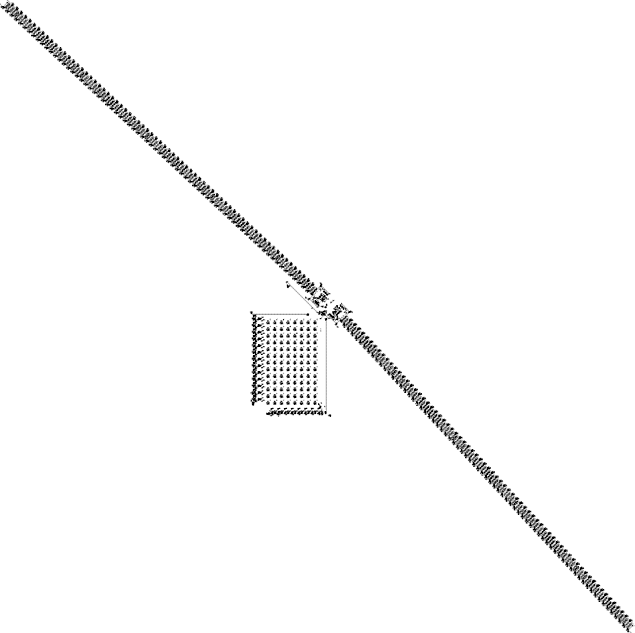
\includegraphics[width=0.8\textwidth]{figures/UTM.png} % Placeholder for actual UTM image
   \caption{A UTM in Life \cite{Goucher_2011_UTM}}
  \label{fig:utm-in-life}
\end{figure}

\subsubsection{Implications: Turing Completeness of Life}
The theoretical demonstration that a Universal Turing Machine (UTM) can be constructed within the framework of Conway's Game of Life serves as the definitive proof of the system's \textit{Turing completeness}.

\begin{definition}[Turing Completeness in Conway's Game of Life]
Conway's Game of Life is Turing complete if there exists a method to encode any Turing machine $M$ and its input $w$ as an initial configuration (pattern) $P_{M,w}$ on the Life grid such that the evolution of $P_{M,w}$ under the rules of Life simulates the computation of $M$ on $w$. Specifically, the eventual state or behavior of the pattern $P_{M,w}$ (e.g., reaching a stable state, exhibiting periodic behavior, growing infinitely in a specific manner) corresponds directly to the outcome of $M$'s computation (halting and accepting, halting and rejecting, or looping).
\end{definition}

The constructability of a UTM within Life fulfills this definition. It implies that any algorithmic process that can be described and executed by any Turing machine—the standard theoretical model for computation—can, in principle, be simulated by observing the evolution of a sufficiently large and complex initial pattern within Conway's Game of Life. The game's simple local rules give rise to emergent behavior capable of universal computation.

A profound consequence of Turing completeness is the inheritance of undecidability. Since UTMs can simulate any Turing machine, they are subject to fundamental limitations, most famously exemplified by the \textit{Halting Problem}. The Halting Problem asks whether it is possible to determine, for an arbitrary Turing machine $M$ and input $w$, if $M$ will eventually halt on input $w$. Alan Turing proved that no general algorithm (no Turing machine) can solve the Halting Problem for all possible $M$ and $w$. Because a UTM constructed in Life can simulate any $M$, this undecidability translates directly into the domain of Life patterns. It implies that there exist analogous undecidable questions about the long-term behavior of arbitrary initial configurations in Conway's Game of Life.

\subsubsection{Synergy with Universal Construction: Computation Driving Creation}
The concepts of the Universal Turing Machine (UTM) and the Universal Constructor (UC), both realizable within Conway's Game of Life, are deeply intertwined. As originally conceived by von Neumann, the Universal Constructor inherently requires an embedded computational component possessing the capabilities of a Universal Turing Machine. This embedded UTM serves as the "brain" or control unit of the UC.

The necessity of the UTM arises from the complexity of the construction task. The UC must read and interpret a potentially arbitrarily complex blueprint, $\mathcal{D}(M)$, which specifies the machine $M$ to be constructed. This interpretation involves parsing the encoded instructions, calculating target coordinates, sequencing actions, and controlling the physical manipulations performed by the construction arm subsystem. Executing these tasks for any possible blueprint requires a computational device capable of universal computation—precisely the function of a UTM. Without the UTM's ability to process any algorithm encoded in the blueprint, the constructor would be limited to building only a predefined set of structures, failing the requirement of universal construction.

Therefore, a system within Conway's Game of Life that can host a Universal Constructor implicitly demonstrates the capacity to host a Universal Turing Machine. The combined potential represents a remarkable level of emergent complexity within the cellular automaton framework. Such a system possesses not only the power to simulate any computation (via the UTM) but also the power to physically realize any constructible design, including itself (via the UC directed by the UTM). This synergy mirrors, at a theoretical level, fundamental aspects of biological systems which combine complex information processing (computation) with physical self-organization and reproduction (construction).

In conclusion, the ability to construct a UTM within Conway's Game of Life is not merely an endpoint demonstrating Turing completeness. It is also a foundational prerequisite for achieving the more ambitious goal of universal construction and, consequently, non-trivial self-replication within the same formal system. The UTM provides the necessary computational engine that drives the creation process specified by the blueprint.

As a final note, let's consider what can't be decided with a traditionally defined UTM? The proof is far too long for this already verbose write-up, but it turns out PREP on an \textit{infinite} grid is \textit{precisely} an analog of the Halting Problem in GoL.

\printbibliography

\end{document}
